\section{ФУНКЦИОНАЛЬНОЕ ПРОЕКТИРОВАНИЕ}
\label{sec:functional}

В данном разделе рассматривается проектирование системы на функциональном уровне, в
соответствии с полученной ранее структурной схемой. Для обеспечения модульности,
на данном уровне используются IP-ядра и стандартизированные протоколы обмена данными
между ними.

Разработка устройств на FPGA заметно облегчается механизмом IP-ядер (\en{Intellectual Property}) --- готовых
блоков для проектирования микросхем и прочих цифровых устройств. IP-ядра представляют собой
конфигурируемый блок цифрового устройства, описанный на HDL (\en{Hardware Description Language}).
Как правило, разработчик IP-ядра включает в него широкий перечень изменяемых параметров,
позволяя сторонним разработчикам переиспользовать ядро в своих целях, внося минимум необходимых
изменений вручную.

\subsection{Структура системы}
\label{sec:functional:structure}

Разрабатываемая система разделена на несколько блоков:

\begin{itemize}
  \item Video In to AXI4-Stream --- блок преобразования видеопотока в \en{AXI4-Stream};
  \item VDMA IN --- Video DMA для входного видеопотока;
  \item Memory Interface Generator --- контроллер DDR-пямяти;
  \item VDMA OUT --- Video DMA для выходного видеопотока;
  \item AXI CLKGEN --- генератор тактового сигнала для контроллера \en{HDMI};
  \item AXI HDMI TX --- блок управления контроллером \en{HDMI};
  \item AXI Camera I2C --- блок управления камерой посредством I2C;
  \item AXI HDMI I2C --- блок конфигурации контроллера \en{HDMI} посредством \en{I2C};
  \item AXI UART-Lite --- блок контроллера \en{UART};
  \item MicroBlaze --- soft-core микропроцессор для управления работой блоков;
  \item MicroBlaze Debug Module --- отладочный модуль для \en{MicroBlaze};
  \item MicroBlaze Local Memory --- локальная память \en{MicroBlaze};
  \item Processor System Reset --- контроллер сброса системы.
    % Докинуть сюда контроллер прерываний
    % Interconnect?
\end{itemize}

Чертёж системы приведён ГУИР.400201.064 Э2.

\subsection{Video In to AXI4-Stream}
\label{sec:functional:video_in_to_axi4stream}
Большинство IP-ядер нацеленные на обработку видео используют протокол AXI4-Stream для
обмена данных. Передача видео между системами, обычно, сопровождается сигналами гашения и
синхросигналами для указания вертикальной и горизонтальной синхронизации, а также
валидности данных в видеопотоке. Интерфейс DVI (Digital Visual Interface) является
одним из представителей такого режима передачи. Ядро Video In to AXI4-Stream преобразует
входящий видеопоток и его управляющие и синхросигналы в протокол AXI4-Stream для
связи с другими блоками, поддерживающими данный протокол. На вход блоку поступает
видеопоток в параллельном виде, частота прорисовки одного пикселя и следующий набор
тайминговых сигналов:

\begin{itemize}
  \item Vsync, Hsync, Data Valid;
  \item Vblank, Hblank, Data Valid;
  \item Vsync, Hsync, Vblank, Hblank, Data Valid.
\end{itemize}

Для полноценной работы блока достаточно любого из этих трёх наборов сигналов. Выбор конкретного
множества существеннен при исползовании детектора Video Timing Controller.
Внутреннее устройство блока представлено на рисунке~\ref{fig:functional:vid_in_to_axi4stream:inner_structure}

\begin{center}
  \centering
  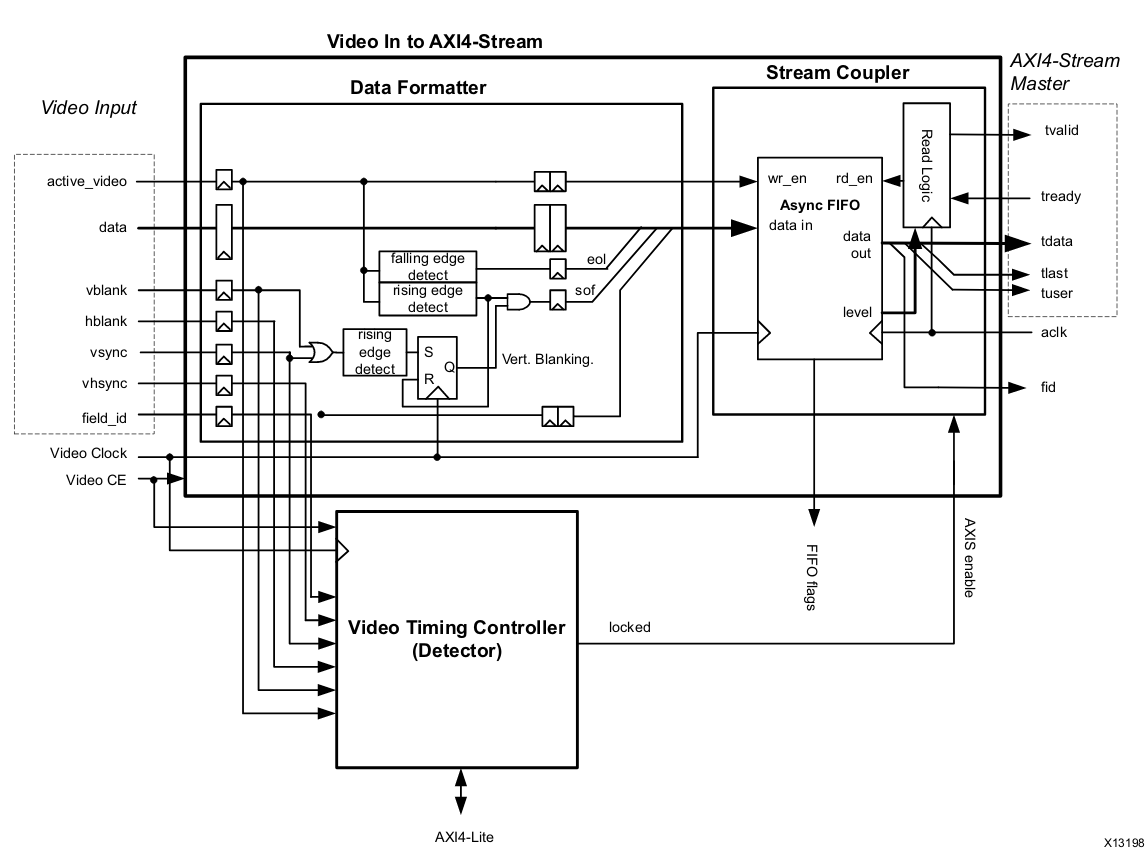
\includegraphics[scale=0.4]{vid_in_to_axi4stream.png}
  \captionof{figure}{ Структурная схема ядра Video In to AXI4-Stream }
  \label{fig:functional:vid_in_to_axi4stream:inner_structure}
\end{center}

Описание сигналов общего назначения:

\begin{itemize}
  \item ACLK --- тактовый сигнал шины AXI4-Stream, входной видеосигнал сэмплируется по фронту
    тактового импульса, выходной сигнал \en{AXI4-Stream} изменяется через некоторое время после фронта ACLK;
  \item ACLKE --- разрешение тактирования, активный высокий уровень. В случае подачи низкого уровня
    приостанавливает работу выходной шины, сохраняя внутреннее состояние блока. При переходе
    из низкого уровня в высокий входной видеопоток не сэмплируется, таким образом подавляя перезаписывание
    кадра в памяти блока.
  \item VCE (Video Clock Enable) --- разрешение работы внутренних регистов, отвечающих за работу с видео.
    Используется, когда видеосигнал подаётся с большей частотой, чем подразумевает стандарт синхронизации видео.
\end{itemize}

Описание видеосигналов приведено в таблице~\ref{table:functional:vid_in_to_axi4stream:video_signals}

\begin{table}[ht]
  \caption{Описание видеосигналов блока Video In to AXI4-Stream}
  \label{table:functional:vid_in_to_axi4stream:video_signals}
  \begin{tabular}{| >{\centering}m{0.18\textwidth}
                  | >{\centering}m{0.17\textwidth}
                  | >{\centering\arraybackslash}m{0.57\textwidth}|}
   \hline
    Обозначение сигнала & Разрядность & Краткое описание \\
    \hline
    ACTIVE & 1 & Валидность видеоданных. 1 --- активный видеопоток,
                        0 --- отсутствие видеоданных \\
    \hline
    DATA & 10 & Параллельный видеопоток \\
    \hline
    HBLNK & 1 & Строчный гасящий импульс, активный высокий уровень \\
    \hline
    HSYNC & 1 & Сигнал горизонтальной синхронизации, активный высокий уровень \\
    \hline
    VBLNK & 1 & Кадровый гасящий импульс, активный высокий уровень \\
    \hline
    VSYNC & 1 & Сигнал вертикальной синхронизации, активный высокий уровень \\
    \hline
  \end{tabular}
\end{table}

Описание сконвертированного видеопотока приведено в таблице~\ref{table:functional:vid_in_to_axi4stream:output_signals}

\begin{table}[ht]
  \caption{Описание выходных сигналов блока Video In to AXI4-Stream}
  \label{table:functional:vid_in_to_axi4stream:output_signals}
  \begin{tabular}{| >{\centering}m{0.18\textwidth}
                  | >{\centering}m{0.17\textwidth}
                  | >{\centering\arraybackslash}m{0.57\textwidth}|}
    \hline
    Обозначение сигнала & Разрядность & Краткое описание \\
    \hline
    TDAT & 32 & Видеоданные, соответствует AXI4-Stream TDATA \\
    \hline
    TVAL & 1 & Валидность видеоданных, соотвествует AXI4-Stream TVALID \\
    \hline
    TRDY & 1 & Готовность Slave-устройства принять данные, соотвествует AXI4-Stream TREADY \\
    \hline
    TLAST & 1 & Сигнал End of Line, соотвествует AXI4-Stream TLAST \\
    \hline
    TUSER & 1 & Начало нового кадра, соотвествует AXI4-Stream TREADY \\
    \hline
  \end{tabular}
\end{table}

По спецификации AXI4-Stream разрядность линий TDATA должна быть кратна 8-ю битам. % Вот тут хер пойми как правильно просклонять
Если входной видеопоток не кратен 8 битам, то данные должны быть дополнены нулями
начиная с старшего значащего бита. Таким же образом упакован выходной видеопоток.
На рисунке~\ref{fig:functional:vid_in_to_axi4stream:packed_output} показан
видеопоток с 12-ю битами на один канал формата RGB.

\begin{center}
  \centering
  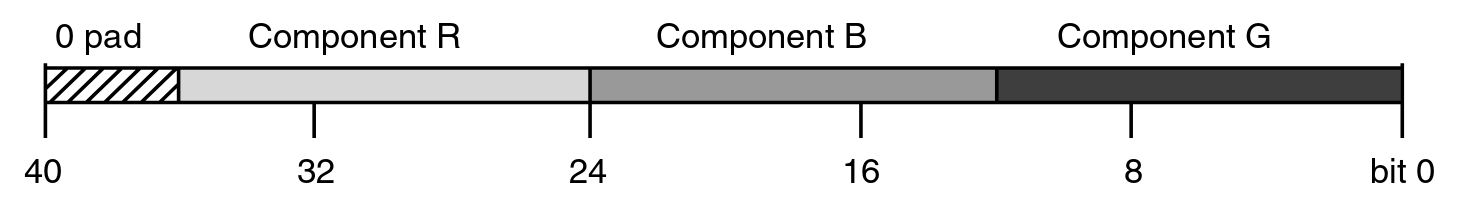
\includegraphics[scale=0.3]{vid_in_to_axi4stream_output.png}
  \captionof{figure}{ Упаковка выходного видеопотока в формате RGB }
  \label{fig:functional:vid_in_to_axi4stream:packed_output}
\end{center}

На входы блока подаётся видеопоток с CMOS-камеры. Для этого ядро конфиругируется в режим
\en{Image Sensor}, выбирается нужная разрядность (в данном случае 10 бит). Так как различные
матрицы выдают цветовые каналы в различном порядке, необходимо сконфигурировать порядок цветовых
каналов во входном видеопотоке.

При подключении камеры линии отрисовки пикселей, вертикальной и горизонтальной синхронизации,
валидности данных подключаются напрямую к контроллеру камеры, на линии VCE и ACLKE подаётся высокий уровень,
линия ACLK к общей линии тактирования системы. Для подачи выского или низкого уровня используется
специальный блок констант.

% Что нибудь ещё про камеру сказануть

\subsection{VDMA IN}
\label{sec:functional:vdma_in}
Для обработки изменений в частоте кадров или изменения их размеров в приложениях
связанных с видеоконтентом используют кадровые буферы. Скоростной обмен между
таким буфером и системой обработки необходим: основные временные затраты
приходятся на передачу блоков данных из буфера и запись в него модифицированных частей кадра.

Ядро VDMA предоставляет возможность для высокоскоростного обмена между \en{AXI4-Stream} видеоинтерфейсом
и стандартным \en{AXI4}, разгружая управляющее устройство от активного контроля передачи.

Блок работает как стандартное устройство DMA, путём записи в регистры размера передаваемого блока данных,
начального адреса записи или чтения и количества циклов повторения операции. Оптимизация подобных
операций на микропроцессоре крайне затруднительна.

Блок VDMA оптимизирован для работы с непрерывным потоком данных, благодаря пакетному режиму передачи.
VDMA, в отличие от AXI DMA, имеет дополнительные линии для поддержки передачи видео без потери
сигналов развёртки и частоты отрисовки пикселей, что в дальнейшем можно использовать для смены частоты кадров.

%Добавить текст, чтобы всё съехало на новый лист
Внутреннее устройство блока представлено на рисунке~\ref{fig:functional:vdma_in:inner_structure}

\begin{center}
  \centering
  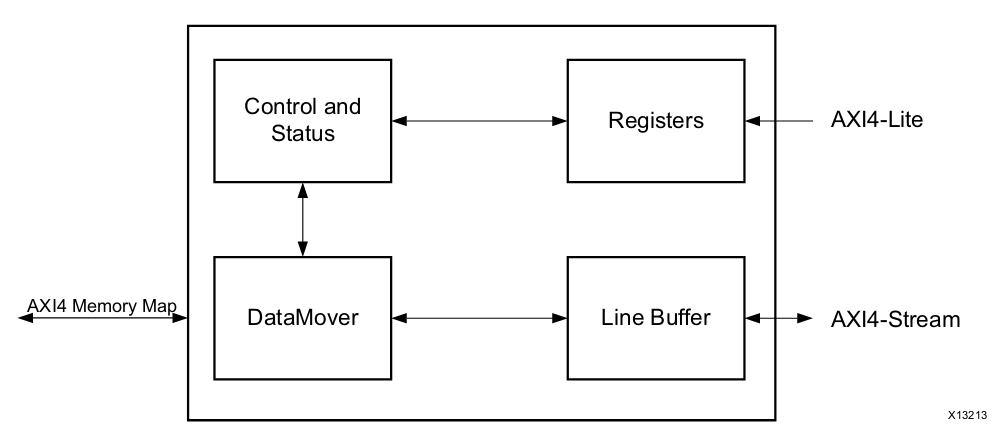
\includegraphics[scale=0.4]{vdma_structure.png}
  \captionof{figure}{ Структурная схема ядра VDMA }
  \label{fig:functional:vdma_in:inner_structure}
\end{center}

После программирования регистров по шине AXI4-Lite, блок управления и состояния генерирует список команд
для блока \en{DataMover}, чтобы инициировать команды чтения и записи интерфейса \en{AXI4 master}.
Асинхронный строковый буфер используется как временное хранилище пикселей с целью их последующей
записи на интерфейс \en{AXI4-Memory Map} или AXI4-Stream.

В случае записи VDMA прингимает кадры по slave интерфейсу AXI4-Stream и записиывает
их в память системы по master интерфейсу AXI4 master. В случае чтения ядро считывает
кадры по master интерфейсу AXI4 из системной памяти и перенаправляет их на master интерфейс
AXI4-Stream. Чтение и запись происходят независимо. Блок поддерживает возможность синхронизировать
входящие или исходящие кадры с внешним тактовым сигналом.

Основные возможности:
\begin{itemize}
  \item совместимость с протоколом AXI4 позволяет использовать модуль в любых приложениях, не разрабатывая
    собственный протокол высокоскоростной передачи данных;
  \item ядро поддеживает разрядность шины AXI4 в 32, 64, 128, 256, 512 и 1024 бита;
  \item ядро поддеживает разрядность шины AXI4-Stream по множителям 8 до 1024 бит;
  \item встроенные 32 кадровых буфера для 32-битного адресного пространства;
  \item опционально используется контроллер автоматического выравниваения обращений к памяти,
    транслируя обращение к произвольному адресу в выровненное. Поддерживается вплоть до 64-битной
    шины \en{AXI4-Stream};
  \item каждый канал VDMA может быть синхронизирован с другим при помощи \en{Genclock}, не позволяя
    при этом обоим каналам обращаться к одному и тому же кадровому буферу;
  \item поддержка асинхронных синхросигналов для различных типов AXI интерфейсов;
  \item блок способен динамически изменять частоту тактирования AXI4-Stream интерфейса,
    что позволяет передавать кадры с частотой и разрешением, отличным от исходных;
  \item поддержка различных механизмов синхронизации кадров, используя пользовательские линии
    шин AXI4.
\end{itemize}

Описание входных сигналов общего назначения приведено в таблице~\ref{table:functional:vmda_in:common_signals}

\begin{table}[ht]
  \caption{Описание входных сигналов общего назначения блока VDMA}
  \label{table:functional:vmda_in:common_signals}
  \begin{tabular}{| >{\centering}m{0.18\textwidth}
                  | >{\centering}m{0.17\textwidth}
                  | >{\centering\arraybackslash}m{0.57\textwidth}|}
   \hline
    Обозначение сигнала & Разрядность & Краткое описание \\
    \hline
    SC & 1 & тактовый сигнал AXI4-Lite \\
    \hline
    S2MC & 1 & тактовый сигнал AXI4-Stream to Memory Map \\
    \hline
    SS2MC & 1 & тактовый сигнал slave AXI4-Stream to Memory Map \\
    \hline
    ARST & 1 & сигнал сброса AXI4-Lite \\
    \hline
    ACLK & 1 & тактовый сигнал шины AXI4-Lite \\
    \hline
  \end{tabular}
\end{table}

Рассмотрим сигналы, используемые во входном VDMA при считывании кадров с преобразователя и последующей их передаче
в оперативную память. Для этого применяется 3 AXI интерфейса: \en{AXI4-Lite} для конфигурации ядра,
slave интерфейс \en{AXI4-Stream} to Memory Map для считывания входящего видеопотока и master интерфейc AXI4
для записи потока в оперативную память. В данном подразделе содержится описание протокола \en{AXI4-Lite}.


AXI4-Lite представляет собой упрощенную версию шины AXI4, без поддержки сложного механизма транзакций,
рассчитанную на задачи не требующие высокой пропускной способности. Благодаря этому контроллер шины
занимает мало места на кристалле микросхемы и обладает простым интерфейсом и принципом работы.

Шина AXI4-Lite, как и её более продвинутая версия, состоит из пяти типов каналов:

\begin{itemize}
  \item канал чтения адреса;
  \item канал записи адреса;
  \item канал чтения данных;
  \item канал записи данных;
  \item канал записи ответа;
\end{itemize}

Данные могут передаваться в двух направлениях, между master и slave одновременно,
при этом размер данных может различаться. Такой механизм обеспечивается раздельными соединениями
для передачи адреса и самих данных. AXI4-Lite поддерживает передачу одного блока данных на транзакцию.
На аппаратном уровне шина использует различные тактовые сигналы для каждой пары master-slave,
что позволяет общаться по данному протоколу физически удалённым устройствам, источники
тактовых сигналов которых могут не совпадать. % Правда?

Пример канала чтения показан на рисунке~\ref{fig:functional:vdma_in:read_axi4lite}

\begin{center}
  \centering
  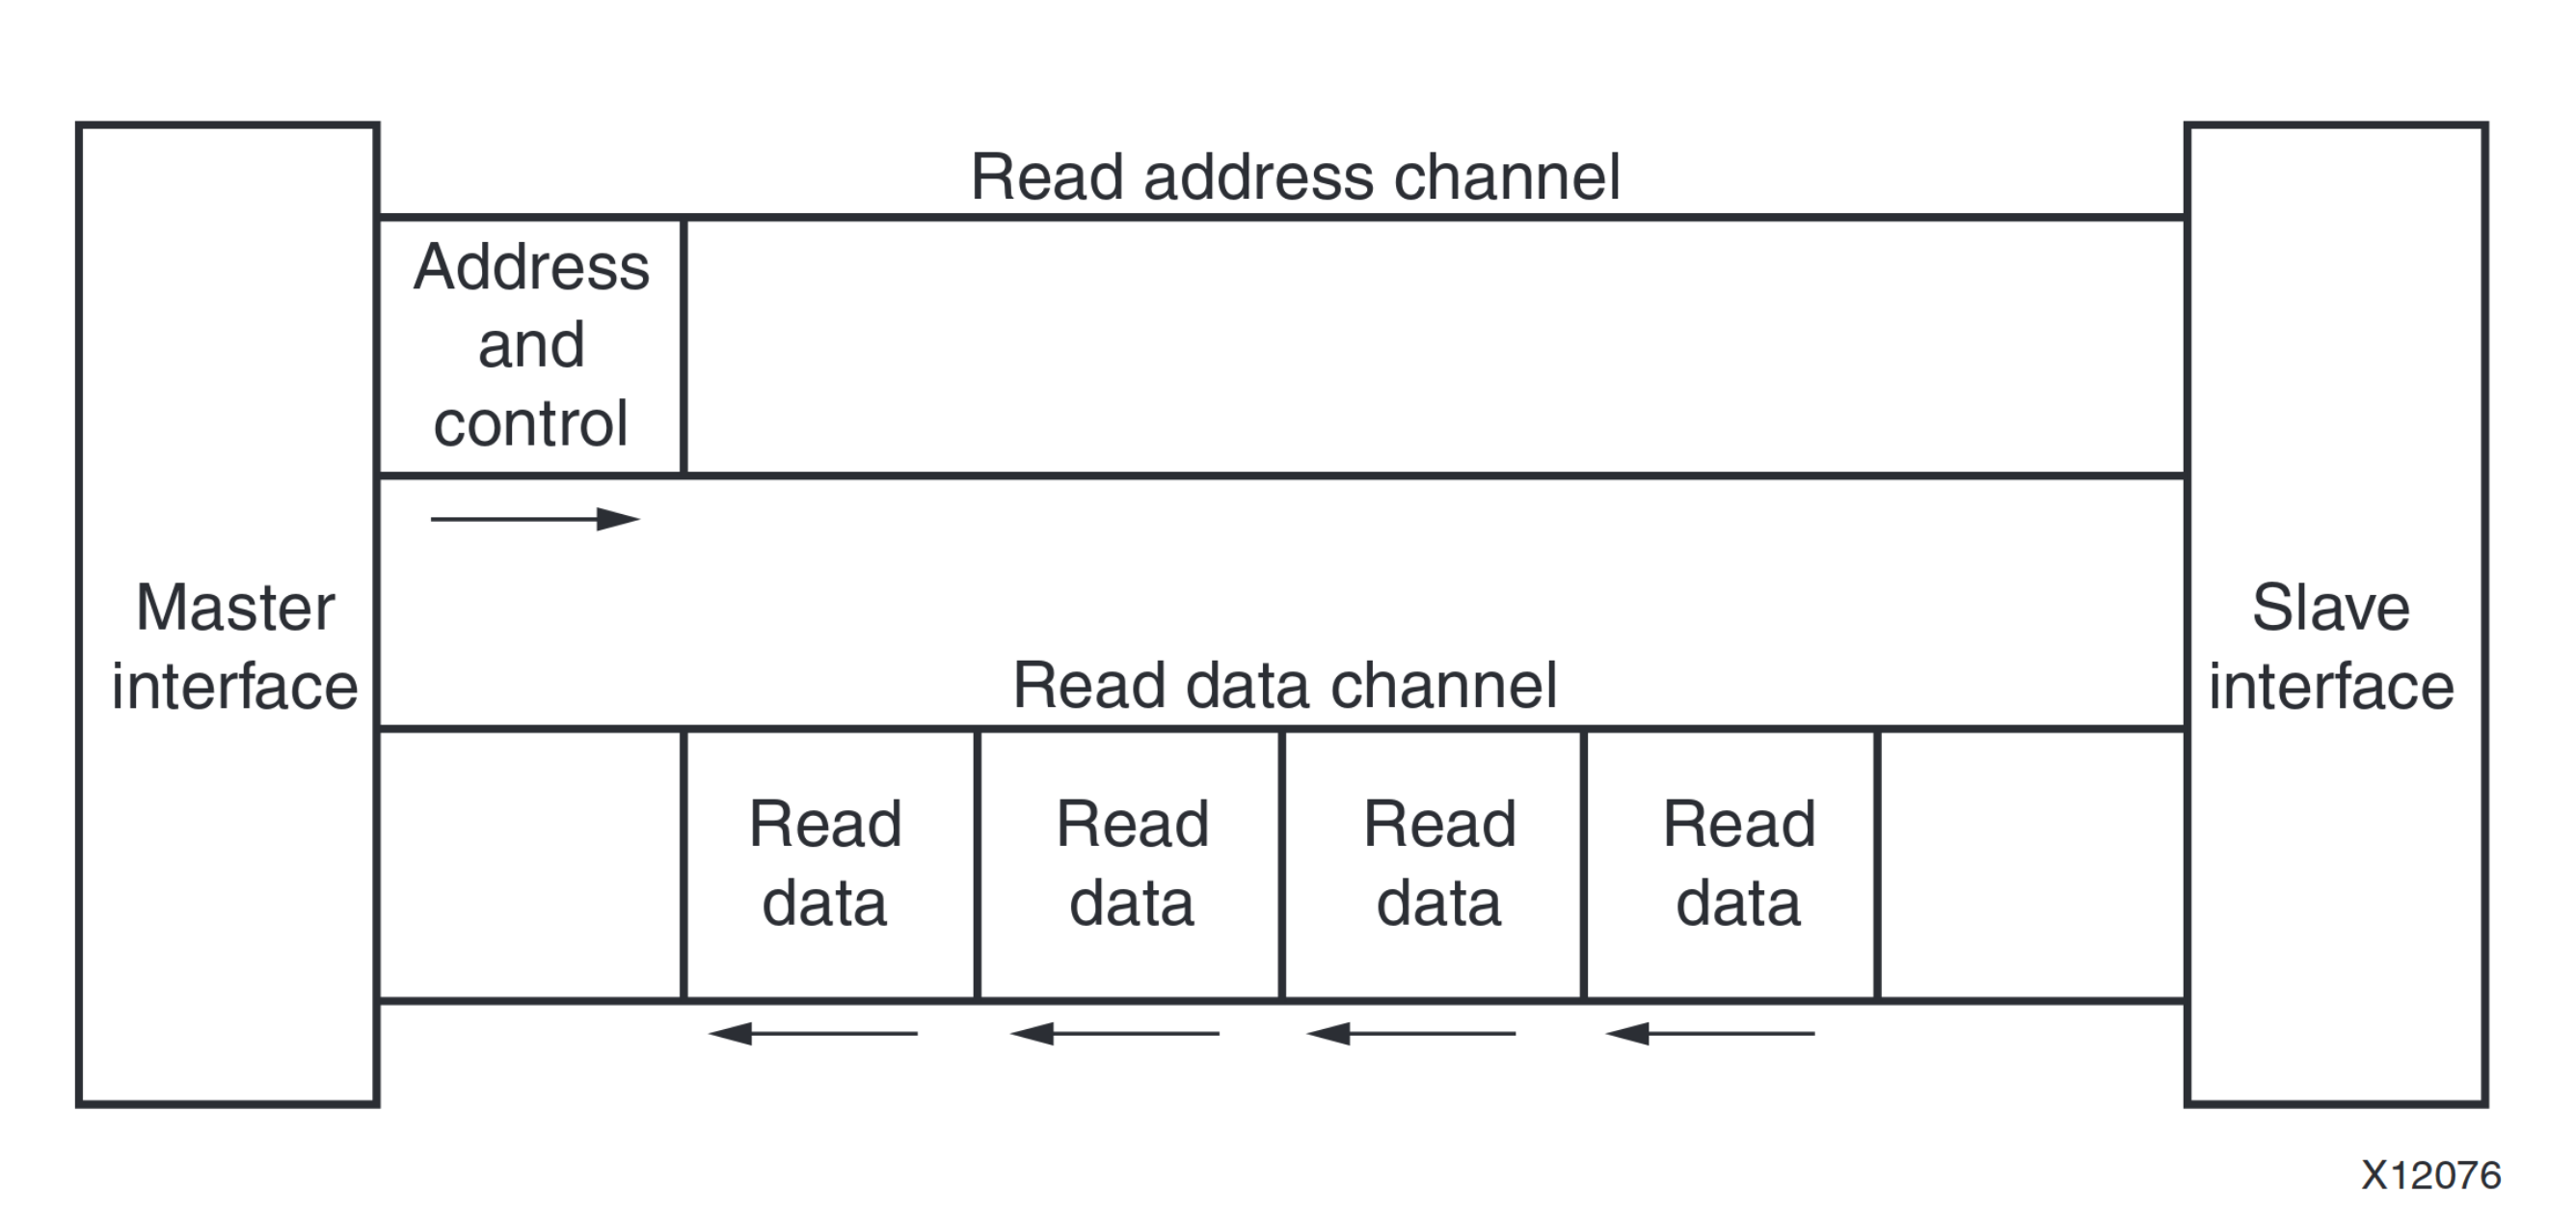
\includegraphics[scale=0.17]{axi4lite_read.png}
  \captionof{figure}{ Канал чтения протокола AXI4-Lite }
  \label{fig:functional:vdma_in:read_axi4lite}
\end{center}

Архитектура канала записи представлена на рисунке~\ref{fig:functional:vdma_in:write_axi4lite}

\begin{center}
  \centering
  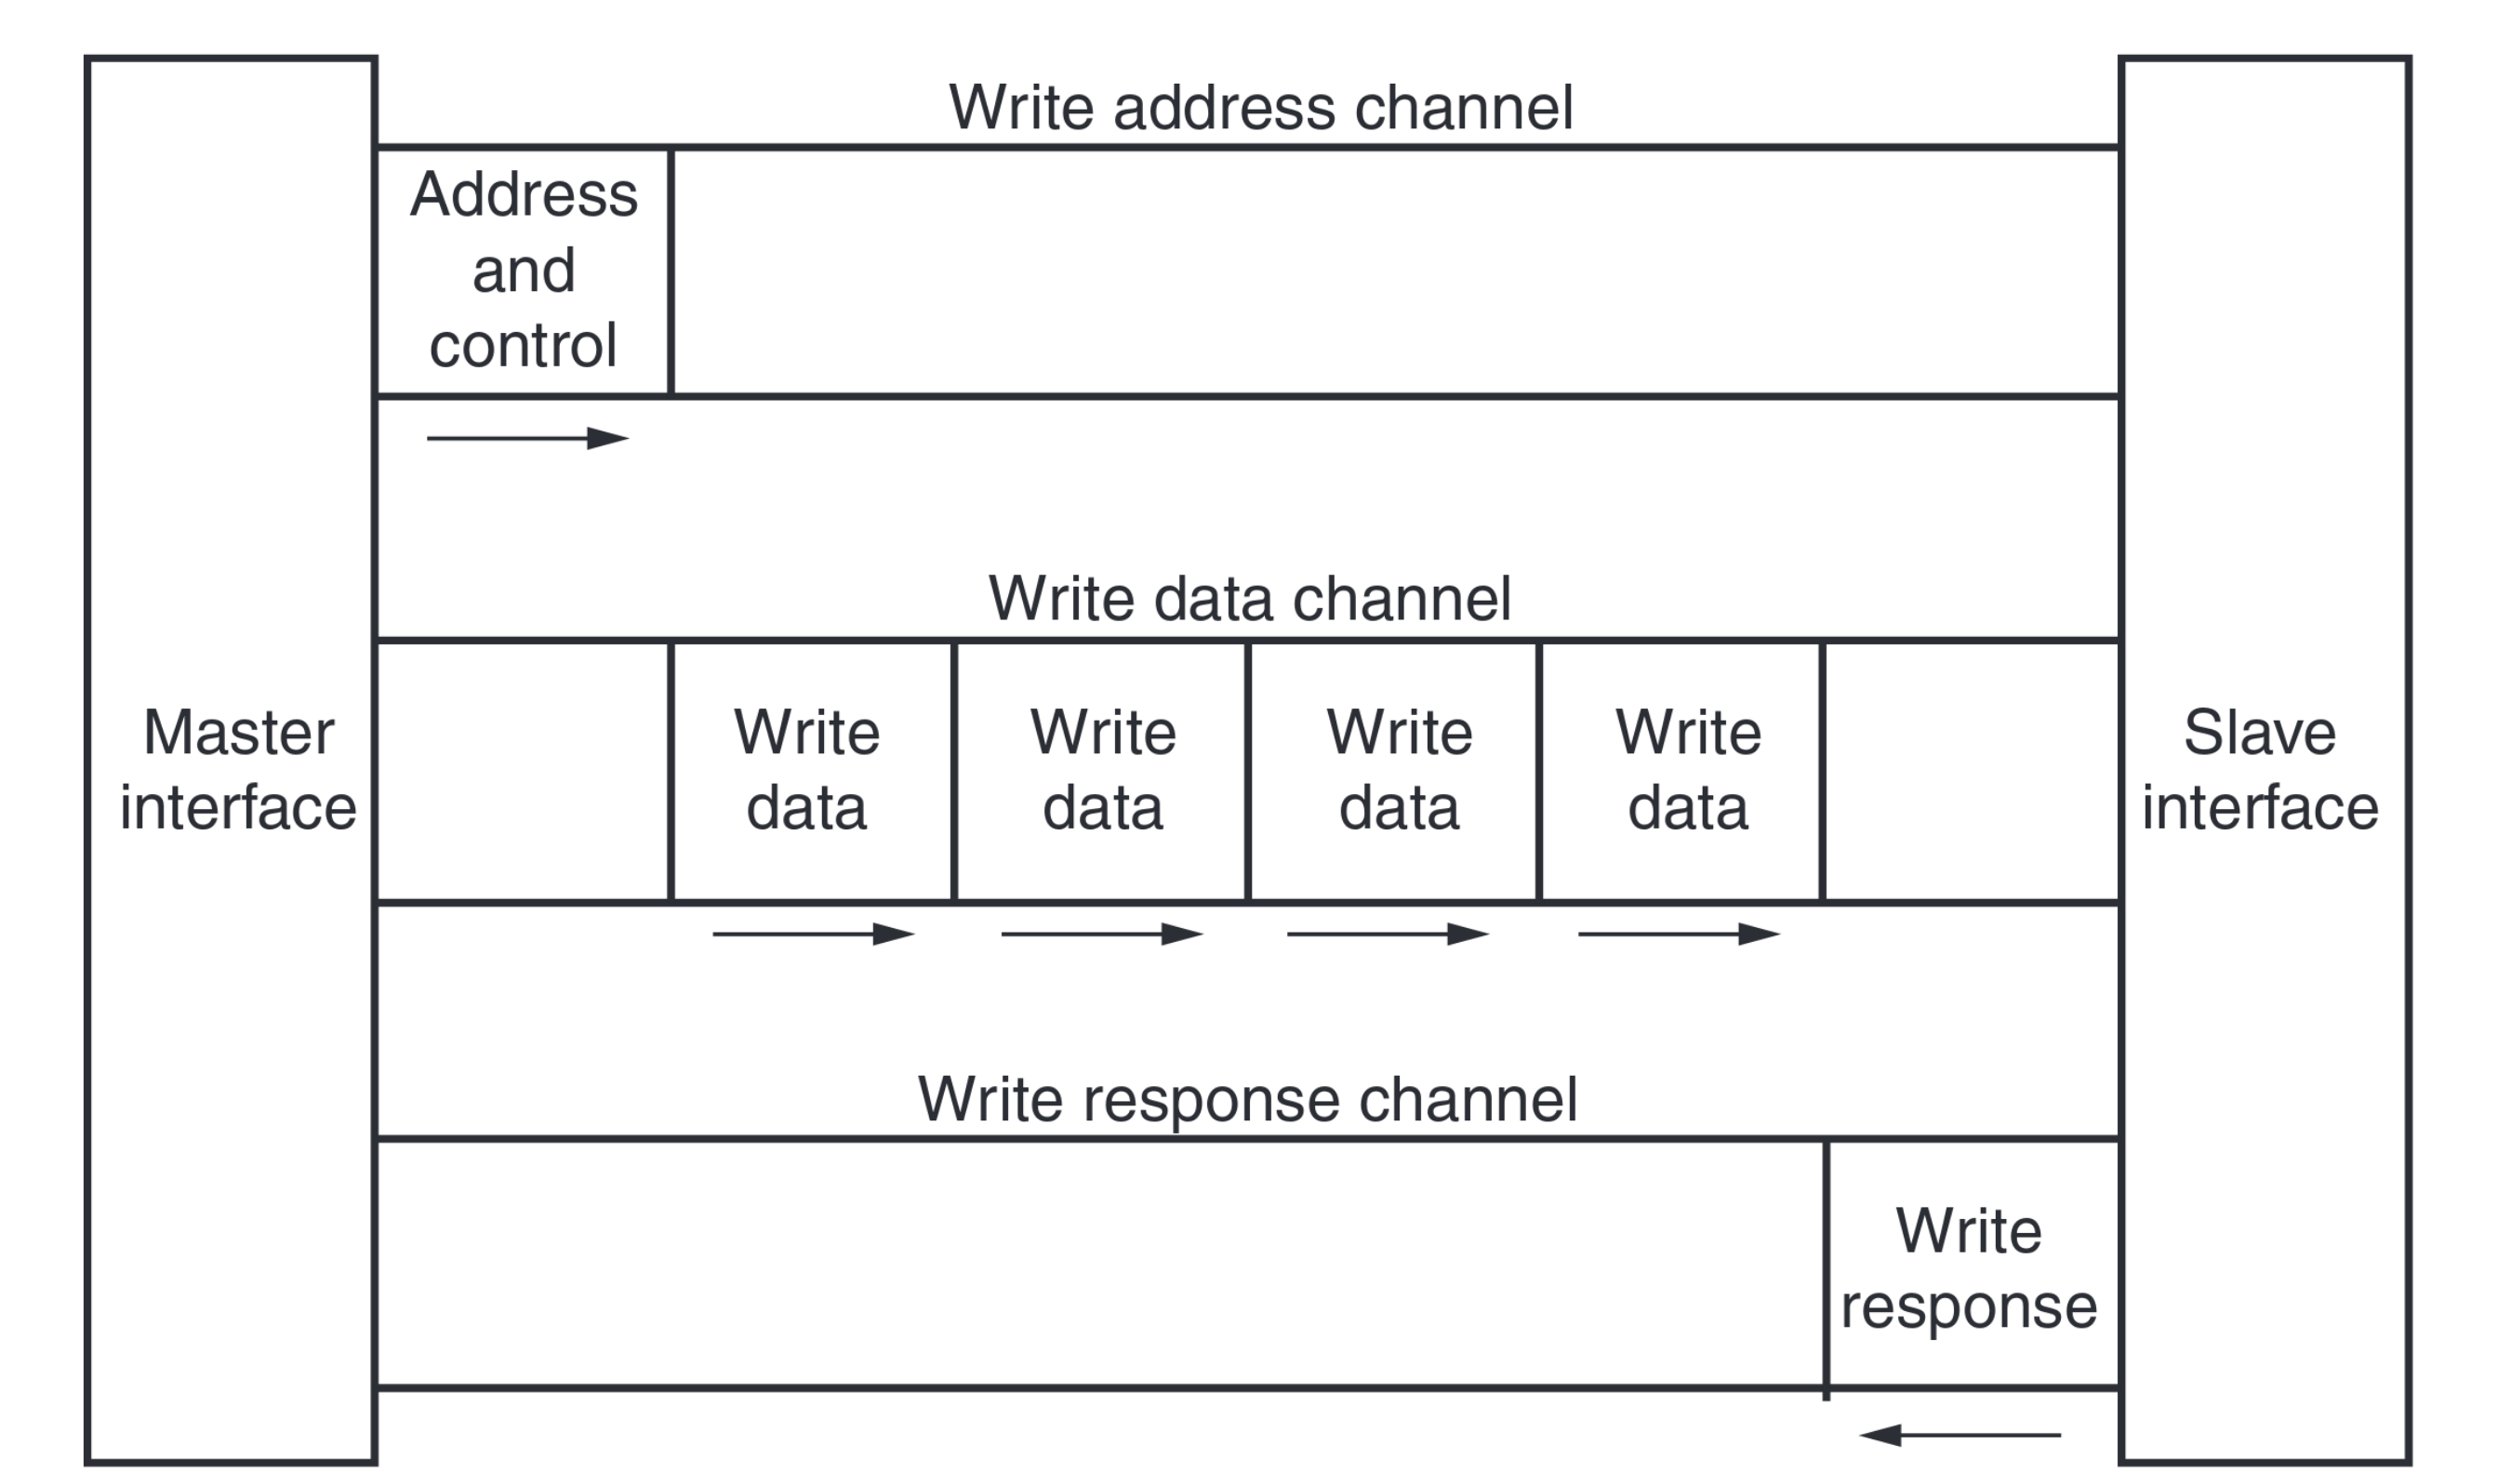
\includegraphics[scale=0.17]{axi4lite_write.png}
  \captionof{figure}{ Канал записи протокола AXI4-Lite }
  \label{fig:functional:vdma_in:write_axi4lite}
\end{center}

Для связи нескольких устройств друг с другом используются блоки \en{AXI-Interconnect},
формируя связи один к одному, один ко многим и многие ко многим.

Выходные сигналы блока VDMA входного потока представляют собой подмножество сигналов AXI4 для
записи данных. Описание сигналов представлено в таблице~\ref{table:functional:vmda_in:output_signals}

\begin{table}[ht]
  \caption{Описание выходных сигналов блока VDMA}
  \label{table:functional:vmda_in:output_signals}
  \begin{tabular}{| >{\centering}m{0.18\textwidth}
                  | >{\centering}m{0.17\textwidth}
                  | >{\centering\arraybackslash}m{0.57\textwidth}|}
   \hline
    Обозначение сигнала & Разрядность & Краткое описание \\
    \hline
    WA & 32 & Адрес записи \\
    \hline
    AWRDY & 1 & Разрешение на запись адреса \\
    \hline
    WVALID & 1 & Валидность данных на шине \\
    \hline
    WD & 64 & Видеоданные \\
    \hline
    DWRDY & 1 & Разрешение на запись данных \\
    \hline
  \end{tabular}
\end{table}

Блок входного VDMA сконфигурирован на режим записи в память. Пример работы
блока в таком режиме представлен на диаграмме~\ref{fig:functional:vdma_in:write_diagram},
путём записи пяти строк по шестнадцать байт.


\begin{center}
  \centering
  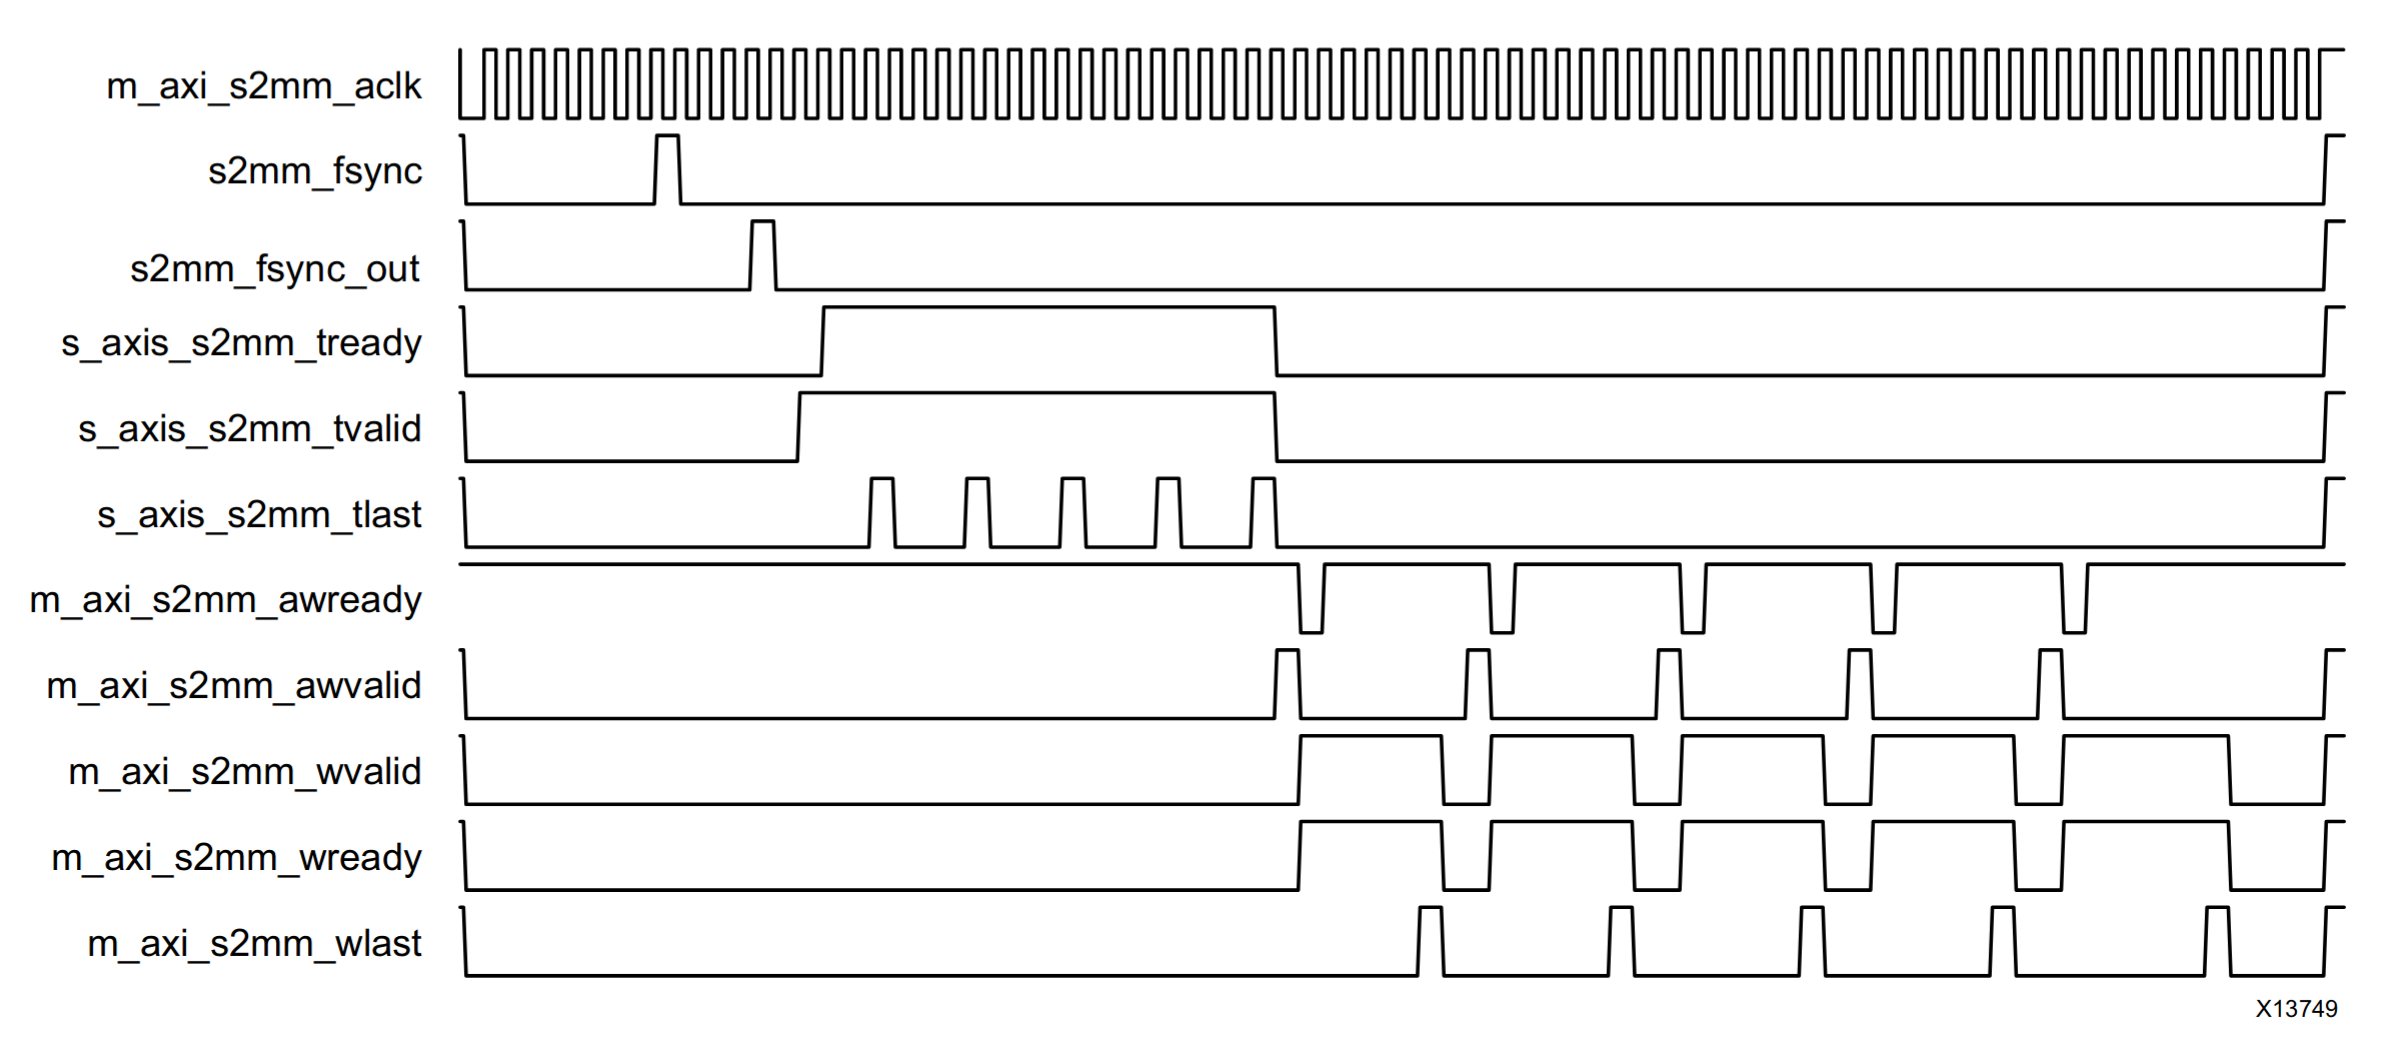
\includegraphics[scale=0.2]{vdma_timing_write.png}
  \captionof{figure}{ Временная диаграмма записи блока данных }
  \label{fig:functional:vdma_in:write_diagram}
\end{center}

Входы блока подключены к выходу преобразователя видеопотока в формат \en{AXI4-Stream}.
Сигналы тактирования и сброса подключены к общим линиям соответствующего назначения. Интерфейс
AXI4-Lite связан с микропроцессором, который производит изначальную конфигурацию, настраивая
режим работы блока. Выходной AXI4 интерфейс подключен к блоку \en{Memory Interface Generator},
управляющий дальнейшей записью видеоданных в оперативную память системы.

% ещё тексту

\subsection{Memory Interface Generator}
\label{sec:functional:mig}

Memory Interface Generator (MIG) представляет собой прослойку, предоставляющую аппаратный и программный
интерфейс взаимодействия с оперативной памятью. Упрощение работы с памятью достигнуто путём сокрытия
интерфейса конкретного типа памяти от разработчика. Упрощённая схема MIG представлена на рисунке~\ref{fig:functional:mig:block_design}

\begin{center}
  \centering
  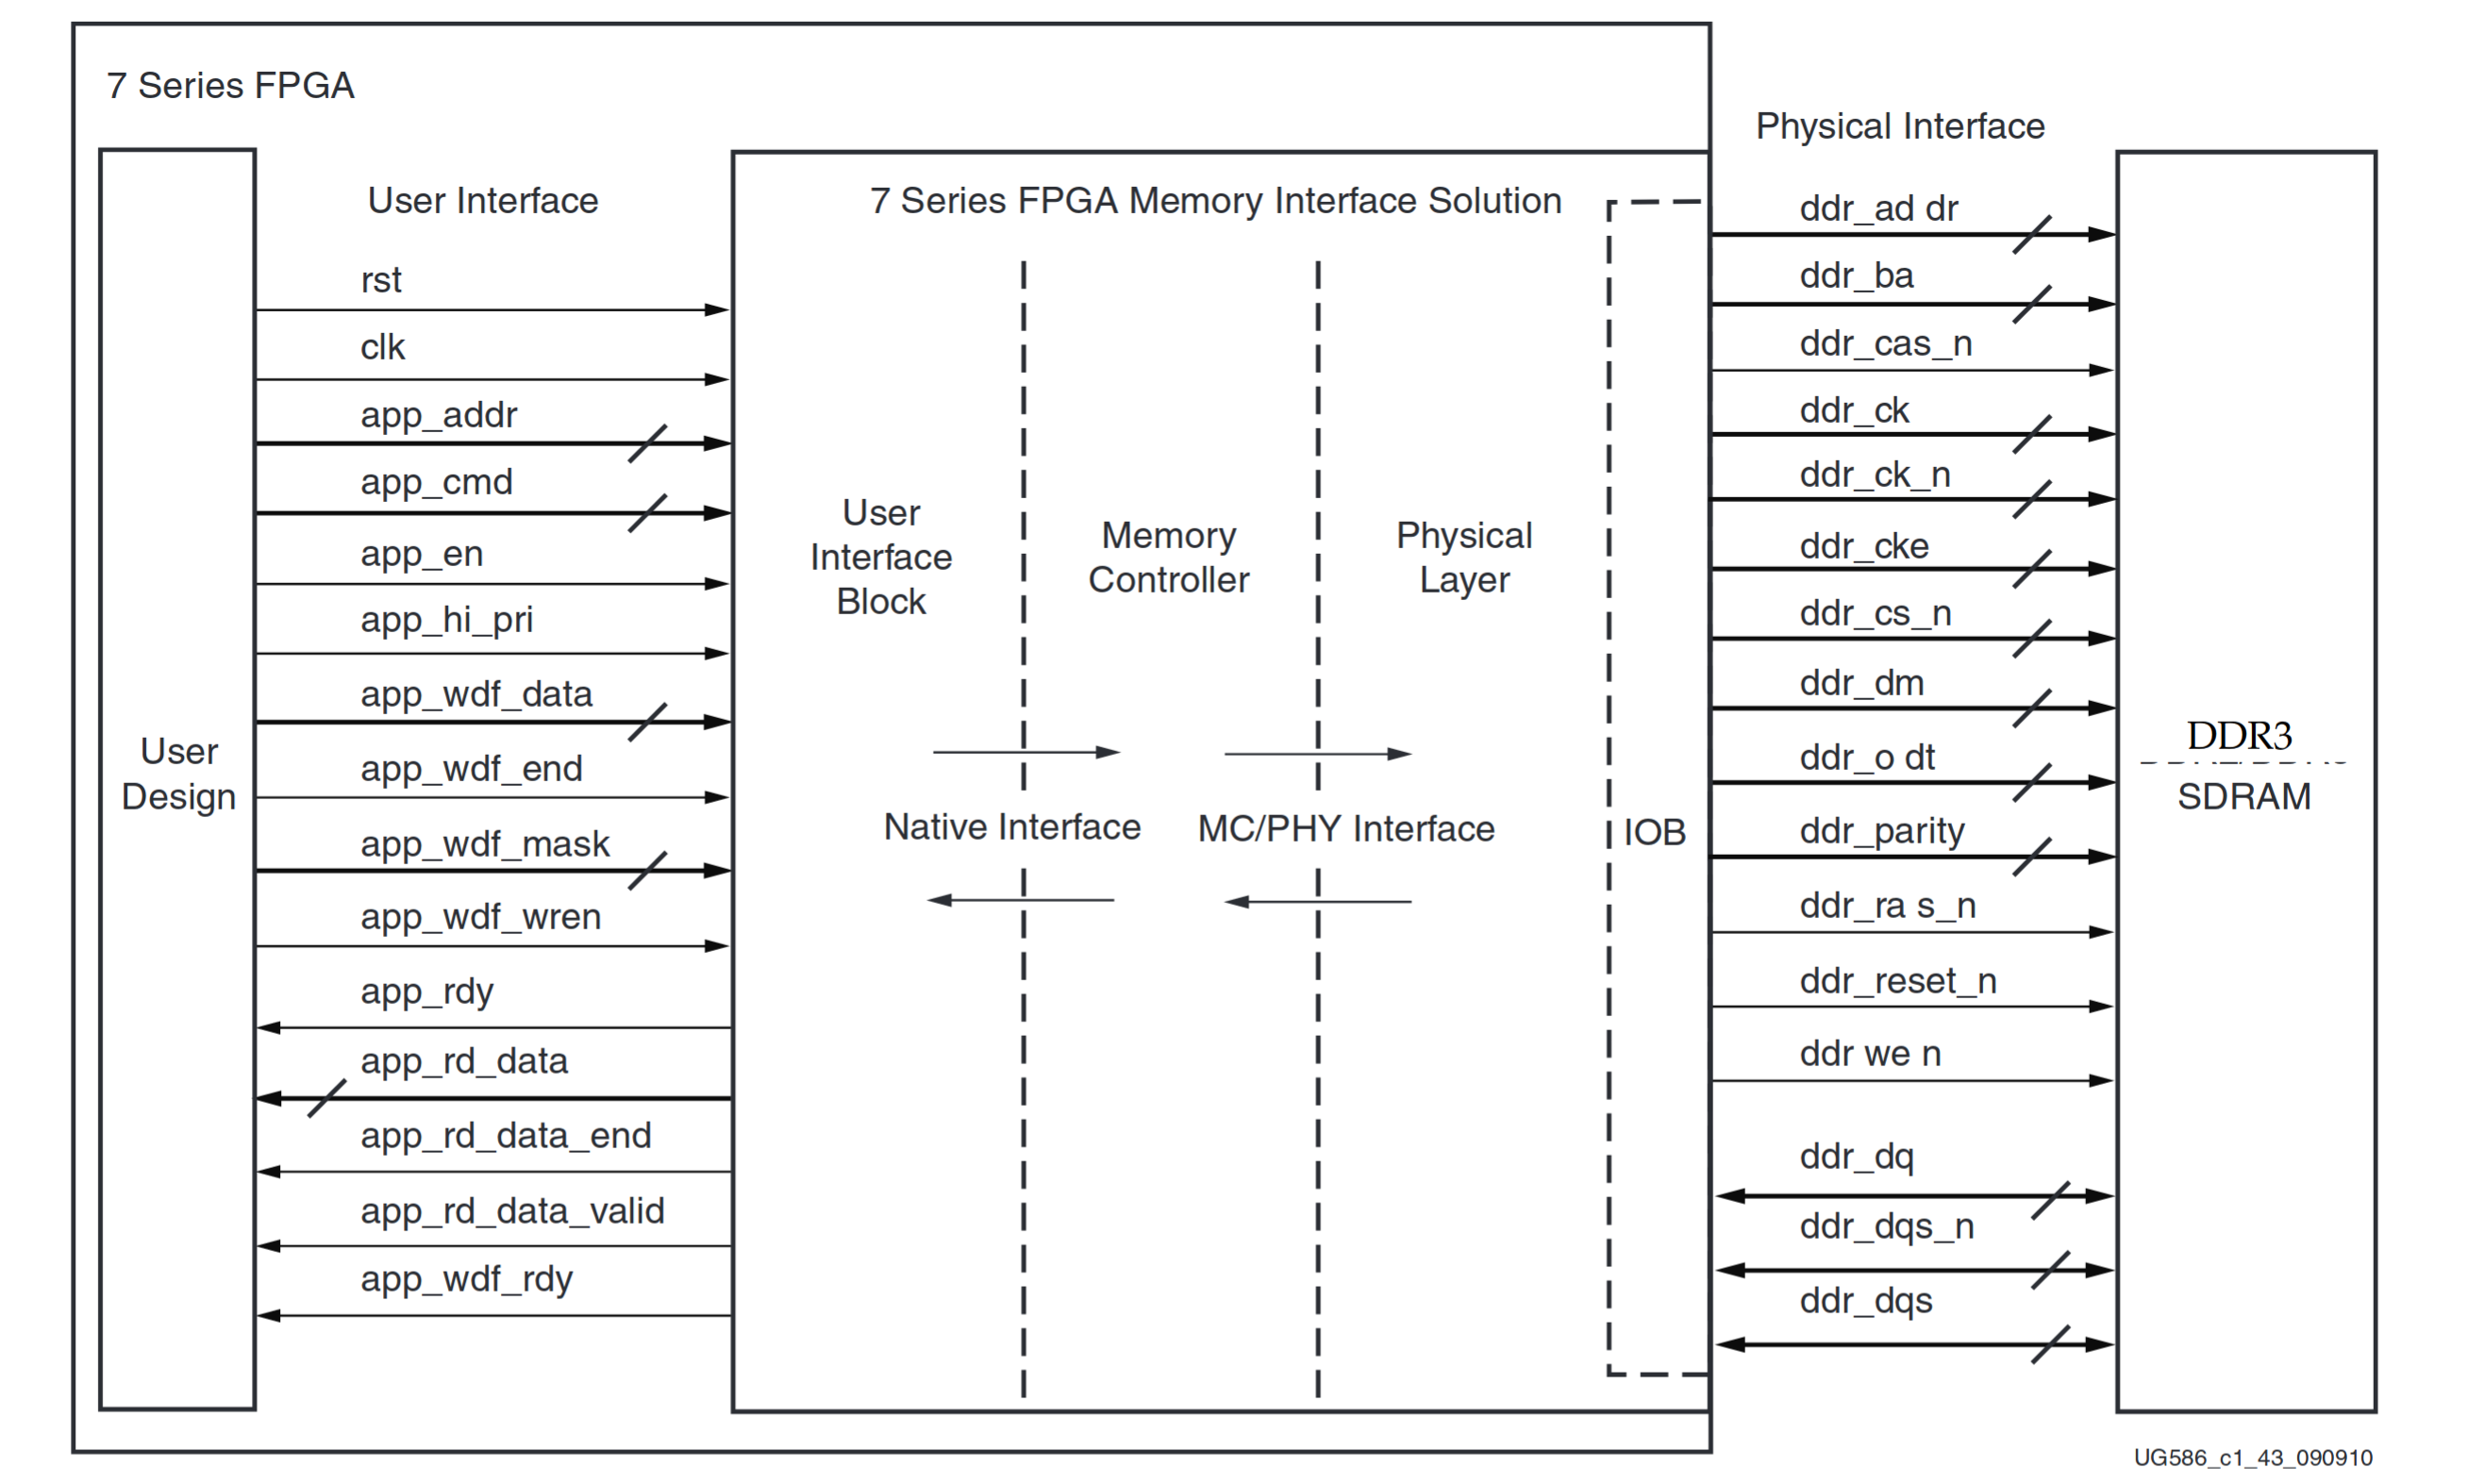
\includegraphics[scale=0.17]{mig_structure.png}
  \captionof{figure}{ Схема устройства MIG }
  \label{fig:functional:mig:block_design}
\end{center}

MIG разбит на несколько блоков. Первый из них это \en{User Design}, представляющий
собой произвольную схему, которая подключается к оперативной памяти \en{DDR3 SDRAM}. Блок связывает
сигналы пользовательской разработки и пользовательского интерфейса MIG. Блок AXI4 slave
соединяет пользовательский интерфейс и контроллер памяти посредством стандартного протокола
AXI4. В свою очередь фронтенд контроллера памяти предоставляет механизмы по чтению и записи
между пользовательским устройством и оперативной памятью, когда бэкенд подключен к физическому
интерфейсу оперативной памяти и обрабатывает все запросы, приходящие от фронтенда. Так же
контроллер может переупорядочивать запросы для улучшения пропускной способности и минимизации
задержек.

В данном случае прослойка \en{User Design} не используется, так как обращение к оперативной памяти
проще всего осуществлять по стандартизированному протоколу AXI4, на базе которого реализована связь
большинства блоков в системе. Интерфейс может конфигурироваться в соответствии со следующими
параметрами:

\begin{itemize}
  \item ADDR\_WIDTH --- разрядность шины адреса для чтения или записи. Принимает значение 32;
  \item DATA\_WIDTH --- разрядность шины данных для чтения или записи. Может принимать значения
    от 32 до 256 по степеням двойки;
  \item ID\_WIDTH --- разрядность идентификатора каналов шины AXI. Принимает значения от 1 до 16 бит;
  \item BURST\_SUPPORT --- поддержка пакетной передачи, Необходим в случае поддержки режима пакетной передачи
    master устройством. Часто выставляется автоматически, если рекомендованная разрядность шины данных
    меньше, чем заданная вручную;
  \item BASEADDR --- настройка начального адреса, на который отображается стартовый адрес slave интерфейса
    AXI4. Заданный адрес отображается на rank 1, bank 0, row 0, column 0. В паре с \en{HIGHADDR} определяет
    доступный объём оперативной памяти. Должен принимать значения степени двойки и вместе с \en{HIGHADDR} выровнен
    кратно 4096 байтам;
  \item HIGHADDR --- настройка конечного адреса, на который отображается конечный адрес slave интерфейса
    AXI4.
\end{itemize}

Так как протокол AXI4 использует независимые каналы адреса чтения и записи, а контроллер памяти
обладает лишь одним каналом, то для доступа к ресурсам используют механизм арбитража.
Протокол AXI4 поддерживает различные режимы арбитража для набиолее эффективного взаимодействия с
другими устройствами на шине, параметры и тип генерируемых данных которых может сильно варьироваться.

Первым видом арбитража служит временное мультиплексирование. Каждому каналу выдаётся одинаковый приоритет,
шина предоставляется арбитром через равные промежутки времени каналом, в порядке поступления запросов к арбитру.

В циклическом виде арбитража каналом выдаётся равный приоритет на захват шины. Порядок предоставления шины
зависит от типа последнего обслуженного запроса: если операцией была запись, то приоритет будет отдан чтению,
и наоборот. Если запросы разных типов возникают одновременно и в очередь ожидания пуста, то предпочтение
отдаётся операции записи.

Арбитр типа \en{Read Priority} обслуживает каналы чтения и записи с равным приоритетам.
Обслуживание записи происходит, если удовлетворяется одно из перечисленных условий:
\begin{itemize}
  \item в очереди ожидания нет запросов на чтение;
  \item starve limit для операций чтения достиг 256. Проверятся только по окончанию пакетной транзакции;
  \item лимит ожидания для чтения достиг 16;
  \item параметр QOS для операций чтения не равен нулю. Проверятся только по окончанию пакетной транзакции.
\end{itemize}

Проверки для операции чтения происходят аналогичным образом.

В арбитраже \en{Read priority with Starve Limit} отдаётся приоритет операциям чтения. Запросы на запись
обрабатываются в случае отсутствия операций чтения в очереди ожидания, либо при достижении
счётчиком \en{read starve limit} конечного значения.

Существует два вида арбитража по записи. В первом случае каналу записи отдаётся приоритет перед чтением,
обработка операции чтения происходит при пустой очереди на запись. Во втором случае номера победителей
сохраняются в регистр \en{WRITE\_PRIORITY\_REG}.

В конфигурации по-умолчанию, контроллер памяти служит прослойкой между блоком \en{User Interface} и физическим
интерфейсом. Более детальное устройство контроллера представлено на рисунке~\ref{fig:functional:mig:mem_controller_scheme}

\begin{center}
  \centering
  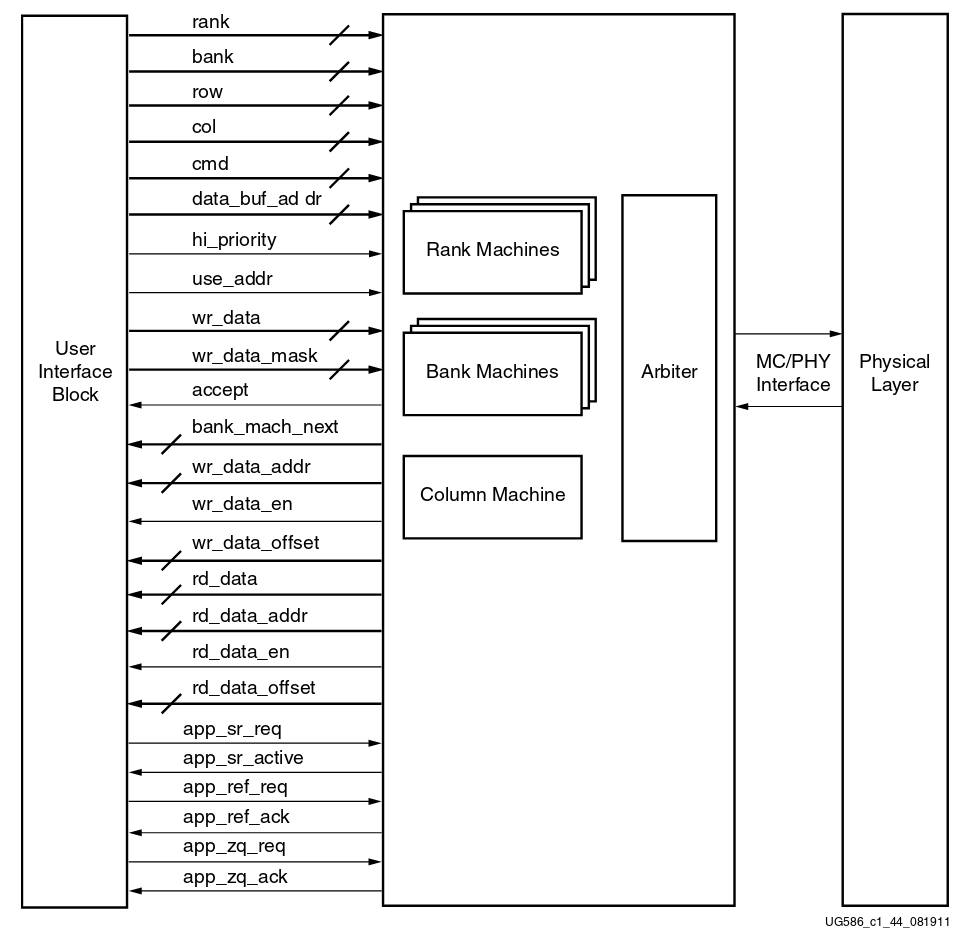
\includegraphics[scale=0.43]{mig_mem_controller.png}
  \captionof{figure}{ Структурная схема контроллера памяти }
  \label{fig:functional:mig:mem_controller_scheme}
\end{center}

Контроллер памяти является главым носителем логики работы MIG. Контроллер сохраняет поступающие от блока \en{User Interface}
в очередь, после чего переупорядочивает их для улучшения производительности.

Блок состоит из четырёх основых частей:
\begin{itemize}
  \item конфигурироемого набора \en{bank} машин;
  \item конфигурироемого набора \en{rank} машин;
  \item машины столбцов;
  \item блока арбитража.
\end{itemize}

Большая часть логики контроллера памяти заложена в блок bank машин. Каждая \en{bank} машина
отвечает за один \en{bank} динамической памяти в любой момент времени. Машины распределяются
динамически, поэтому их соответствие физической памяти не фиксированно. Количество машин
конфигурируется для нахождения баланса между площадью кристала с сгенерированной логикой и
её производительностью.

Время распределения конкретной машины зависит не от состояния соответствующего ей \en{bank}
динамической памяти, а от наличия запросов в память. При поступлении запроса машина
ставится в соответствие с физической памятью, после выполнения всех запросов машина
освобождается и попадает обратно в пул.

Для выполнения запросов машина генерирует команды на чтение или запись строк и столбцов,
которые поступают на физический интерфейс независимо, но соблюдая временнные ограничения.
При возникновении запроса во время простаивания контроллера и оперативной памяти,
\en{bank} машина проиходит следующие этапы:
\begin{itemize}
  \item принимается запрос;
  \item активируется необходимая строка;
  \item выполняется команда на чтение или запись столбца;
  \item указанная строка перезаписывается текущим значением (происходит перезарядка);
  \item машина возвращается в пул.
\end{itemize}

Если в поступившем запросе чтение или запись приходится на уже распределенную машину,
то этап перезаписи строки пропускается, и машина находящаяся в пуле сразу приступает
ко второму этапу обработки.

\en{Rank} машины статически отображаются на \en{rank} оперативной памяти и служат
мониторами активности \en{bank} машин. Они замеряют тайминговые параметры, специфичные
для конкретной оперативной памяти, и в случае выхода за их пределы деактивируют \en{bank}
машины на определенный промежуток времени, для восстановления параметров.

Машины столбцов генерируют тайминговую информацию, необходимую для управления \en{DQ}
шиной. При генерации информации машины столбцов в пределах одной \en{rank} машины
рассматриваются как единое целое. Машины столбцов отслеживают команды, посылаемые
\en{bank} машинами, и генерируют сигналы задержки для \en{bank} машин таким образом, чтобы запросы
к \en{DQ} шине приходили упорядоченно.

Блок арбитража посылает команды от \en{bank} машин к динамической памяти. Команды на чтение и запись
арбитрируются независимо. Для каждого обращения к памяти арбитр выбирает команду по работе со строкой
и столбцом и отправляет их на физический инетрфейс. Блок арбитража работает по циклическому алгоритму.

Блок физического интерфейса предоставляет логику, по работе с внешним \en{DDR2} или \en{DDR3 SDRAM}.
Интерфейс генерирует тайминговые и управляющие сигналы для корректной работы памяти. Он содержит
тактовую, адресную и управляющую логику, набор шин для обмена данными с памятью и логику хранения
состояния устройства. Стурктурная схема блока представлена на рисунке~\ref{fig:functional:mig:phy_scheme}

\begin{center}
  \centering
  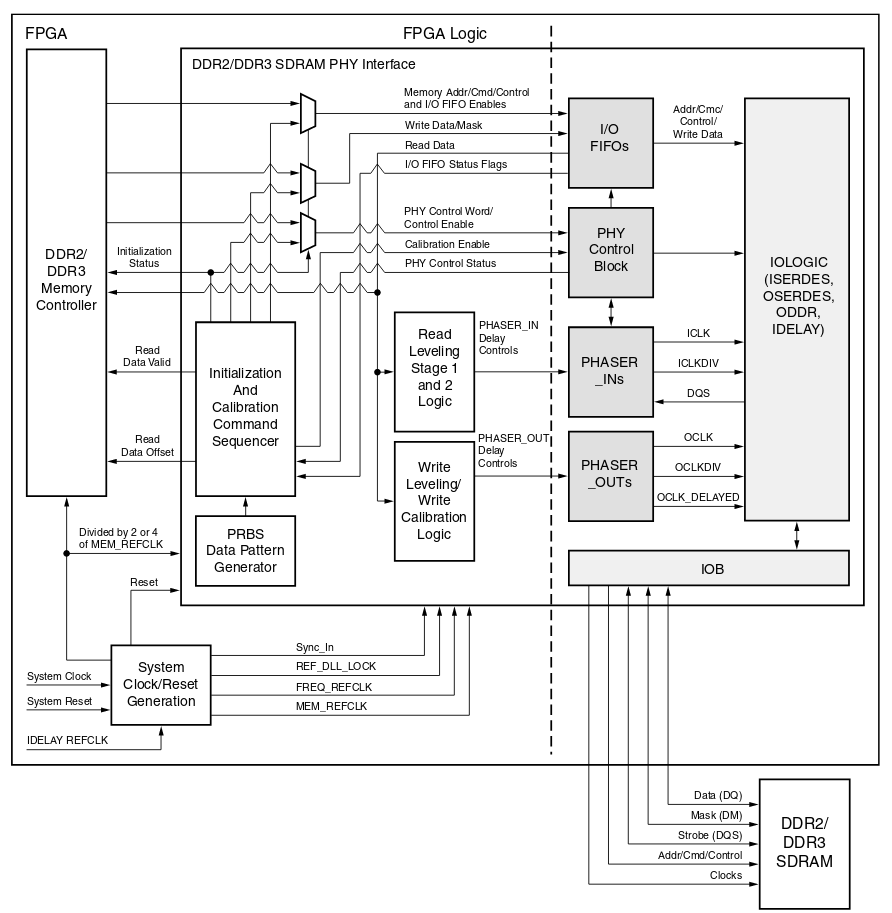
\includegraphics[scale=0.5]{mig_phy.png}
  \captionof{figure}{ Структурная схема физического интерфейса }
  \label{fig:functional:mig:phy_scheme}
\end{center}

Линии связи с динамической памятью делятся на несколько групп: шина данных, маска,
линии строб, управляющие и тактирующие линии. Стробирующие линии служат для дополнительной
синхронизации источника и приёмника данных, т.к. скорость передачи данных достаточно высока.
Часть данных линий характерна исключительно для \en{DDR}. Их назначение приведено в таблице~\ref{table:functional:mig:ddr}
% https://media.digikey.com/pdf/Data%20Sheets/Micron%20Technology%20Inc%20PDFs/MT8JTF(128,256)64A_RevB.pdf

\begin{table}[ht!]
  \caption{ Описание сигналов связи с DDR }
  \label{table:functional:mig:ddr}
  \begin{tabular}{| >{\centering}m{0.18\textwidth}
                  | >{\centering}m{0.17\textwidth}
                  | >{\centering\arraybackslash}m{0.57\textwidth}|}
   \hline
    Обозначение сигнала & Разрядность & Краткое описание \\
    \hline
    DQ & 64 & Данные, двунаправленная шина \\
    \hline
    DQSP & 8 & Строб данных, используемый для операции захвата передачи. Выровнен по фронту с считываемыми данными,
               по центру с записываемыми данными \\
    \hline
    DQSN & 8 & Аналогично DQSP, используется при включении режима дифференциальной передачи \en{LOAD MODE} \\
    \hline
    A & 14 & Адресные входы, различные биты в пределах адреса отвечают за дополнительные функции,
             такие как перезарядка строки и т.д.  \\
    \hline
    BA & 3 & Определяет номер \en{bank}, для которого применяются команды считывания, записи, перезарядки\\
    \hline
    CAS & 1 & Строб доступа к столбцу \\
    \hline
    RAS & 1 & Строб доступа к строке \\
    \hline
    WE & 1 & Разрешение записи \\
    \hline
    CKP, CKN & 1 & Дифференциальный тактовый сигнал, выдача данных и их стробирование синхронизирована с
                   пересечением двух дифференциальных сигналов \\
    \hline
    CKE & 1 & Разрешение тактирования \\
    \hline
    CSN & 1 & Сигнал выключения декодера комманд \\
    \hline
    DM & 8 & Маскирование данных \\
    \hline
    ODT & 1 & Включение терминирующего резистора для линий данных и маскирующих линий \\
    \hline
  \end{tabular}
\end{table}

Маска DDR служит для запрета модификации как конкретных бит в передаваемом байте, так и целых групп
бит, в случае передачи в пакетном режиме.

В системе MIG подключается к \en{VDMA IN} и \en{VDMA OUT} по шине AXI4. \en{VDMA IN} инициирует
запись входного видеопотока в динамическую память. Для минимизации задержек при пересылке
используется пакетный режим передачи. Чтение записанных в память кадров осуществляет блок
\en{VDMA OUT}, передавая их на последующие этапы обработки.

\subsection{VDMA OUT}
\label{sec:functional:vdma_out}

Описание блока \en{VDMA OUT} во многом схоже с \en{VDMA IN}, за исключением нескольких пунктов.
Блок считывает информацию из оперативной памяти, поэтому для операций чтения применяются
соотвественные каналы чтения шины AXI4. Временная диаграмма считывания блока данных такого же
объёма, как и в диаграмме~\ref{fig:functional:vdma_in:write_diagram}, приведена на
рисунке~\ref{fig:functional:vdma_out:read_diagram}

\begin{center}
  \centering
  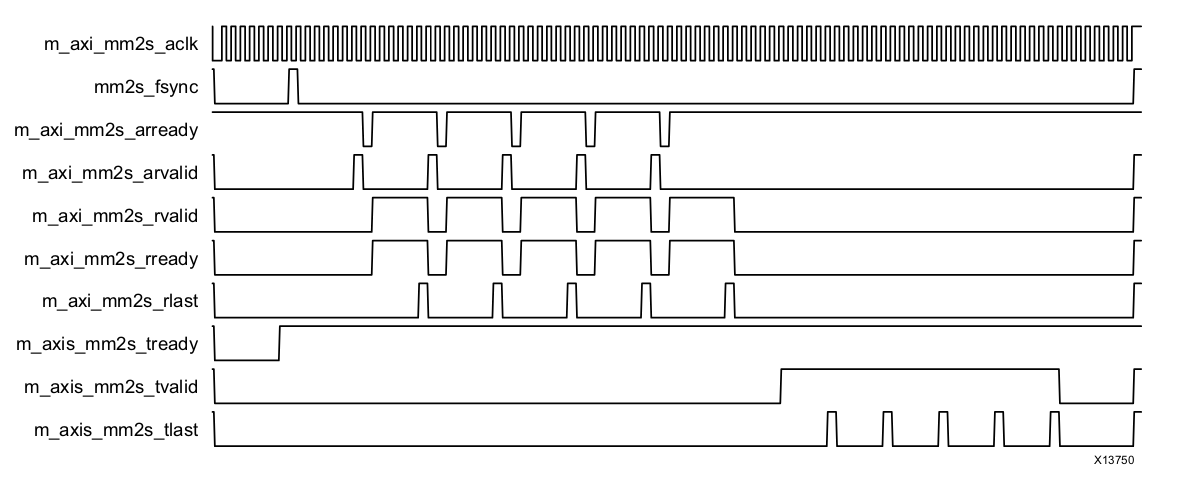
\includegraphics[scale=0.4]{vdma_timing_read.png}
  \captionof{figure}{ Временная диаграмма чтения блока данных }
  \label{fig:functional:vdma_out:read_diagram}
\end{center}

Для упрощения конфигуирирования частоты выдачи кадров на \en{AXI4-Stream} интерфейс в блоке
включена поддержка \en{fsync}. Кадровая синхронизация может принимать следующие значения:
\begin{itemize}
  \item none --- блок выдаёт кадры на максимально возможной частоте, без ожидания внешних
    сигналов-триггеров;
  \item s2mm fsync --- обработка кадров начинается по спаду тактового сигнала \en{s2mm\_fsync};
  \item s2mm tuser --- блок ожидает передачу последовательности \en{start-of-frame (SOF)} по
    шине \en{s2mm\_tuser}. Последовательность совпадает по времени с передачей первого пикселя
    изображения. Задержка перед выдачей пикселя может конфигурироваться при помощи ACLK;
\end{itemize}

VDMA OUT связан с MIG и VDMA IN посредством шины AXI4, в качестве тактовых импульсов для
шины AXI4 используется общий системный тактовый сигнал.
% Пару предолжений организовать

\subsection{AXI CLKGEN}
\label{sec:functional:axi_clkgen}

Блок \en{AXI CLKGEN} представляет собой HAL над MMCM (\en{Mixed-Mode Clock Manager}),
который позволяет создавать тактовые сигналы с заданной фазой и частотой относительно заданного
сигнала. Сам уровень абстракции добавляет дополнительный функционал по конфигурации, необходимой
для взаимодействия с модулем \en{HDMI}. Конфигурация блока осуществляется посредством
протокола AXI4-Lite. Структурая схема блока представлена на рисунке~\ref{fig:functional:axi_clkgen:structure}

\begin{center}
  \centering
  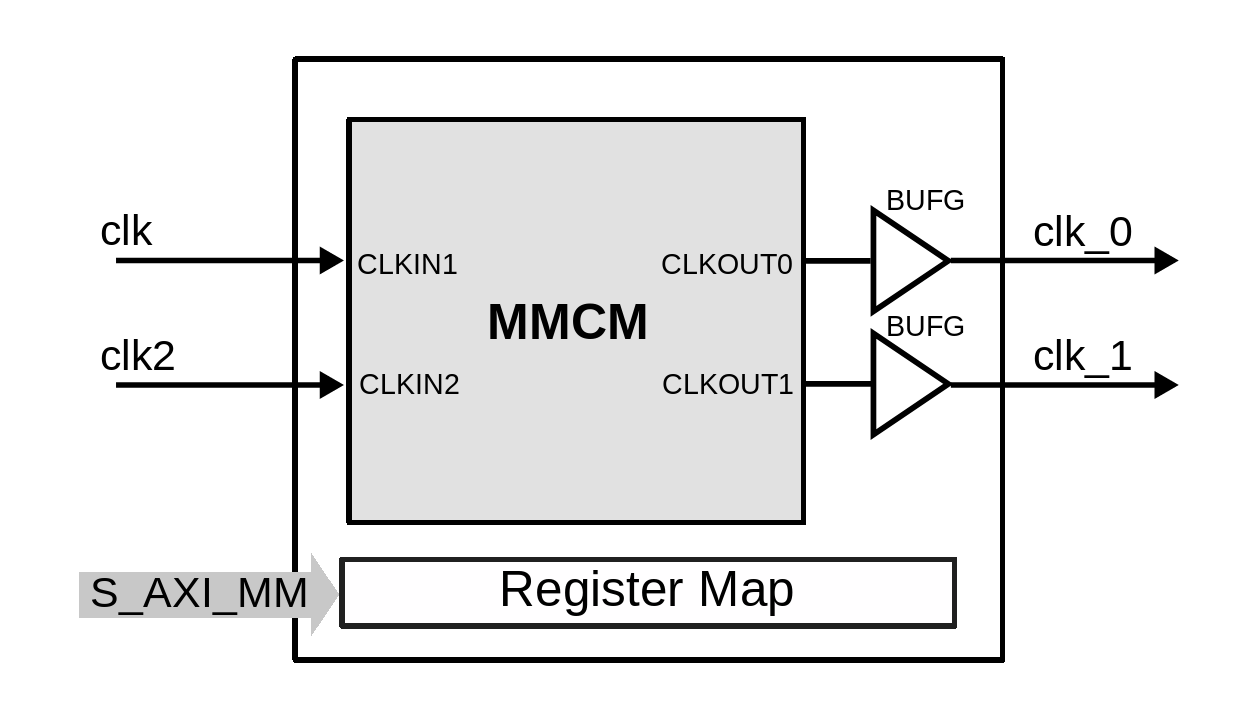
\includegraphics[scale=0.35]{axi_clkgen.png}
  \captionof{figure}{ Структурная схема ядра AXI CLKGEN }
  \label{fig:functional:axi_clkgen:structure}
\end{center}

Блок MMCM выступает в качестве внутреннего генератора тактовых импульсов и позволяет
программно и аппаратно управлять частотой уже используемых генераторов. Детализированная схема
блока управления частотой представлена на рисунке~\ref{fig:functional:axi_clkgen:mmcm_structure}

\begin{center}
  \centering
  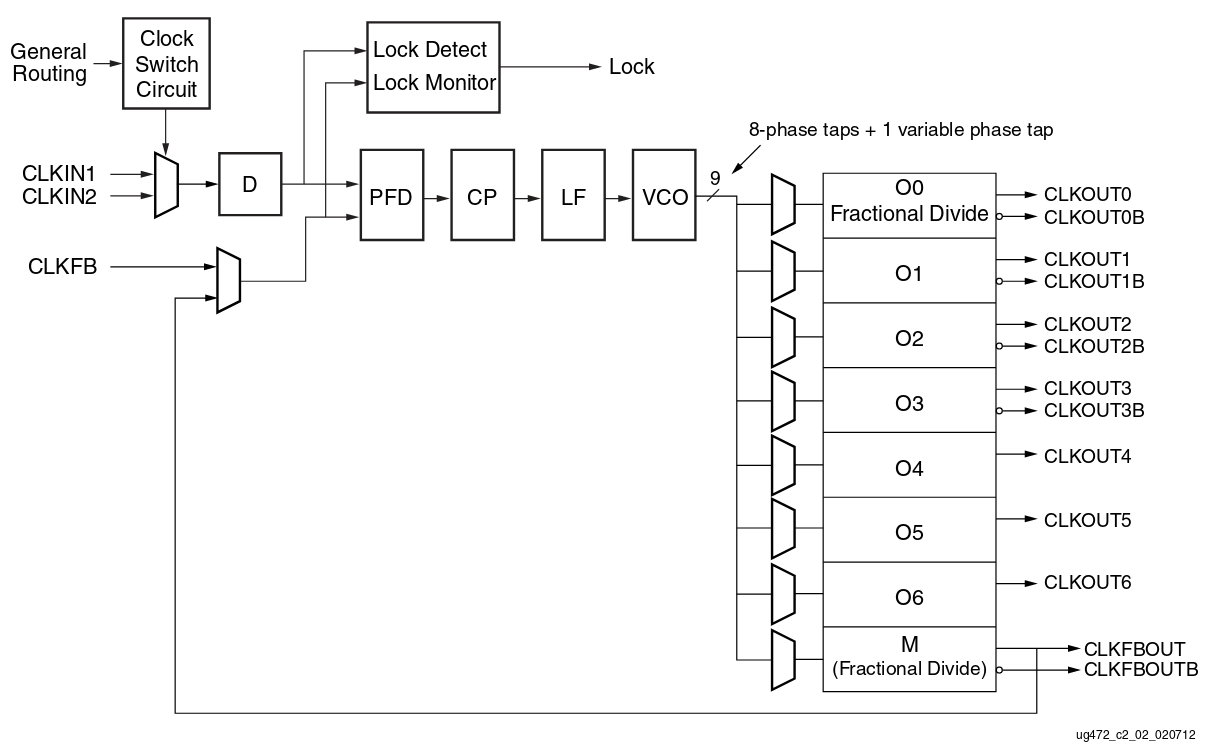
\includegraphics[scale=0.31]{mmcm.png}
  \captionof{figure}{ Структурная схема MMCM }
  \label{fig:functional:axi_clkgen:mmcm_structure}
\end{center}


MMCM поддерживает следующие возможности:
\begin{itemize}
  \item инверсия тактовых сигналов;
  \item параллельная работа шести независимых генераторов тактовых импульсов, часть которых
    может представлять собой дифференциальные сигналы;
  \item динамический сдвиг фазы тактового сигнала;
  \item позволяет избежать рассинхронизации тактовых сигналов, при их передаче на большие
    расстояния, относительно их длины волны. Так же может применяться при плохом качестве
    исходных тактовых импульсов.
\end{itemize}

При применении MMCM в качестве генератора частоты, другие его составные части, такие как
синхронизатор частоты переиспользутся как источник тактовых сигналов. В данном случае
пути тактовых сигналов разведены внутри самого блока, тем самым минимизируя общую длину пути
и джиттер. На рисунке~\ref{fig:functional:axi_clkgen:mmcm_freq_synthesis} представлена
работа MMCM в качестве генератора тактовых сигналов.

\begin{center}
  \centering
  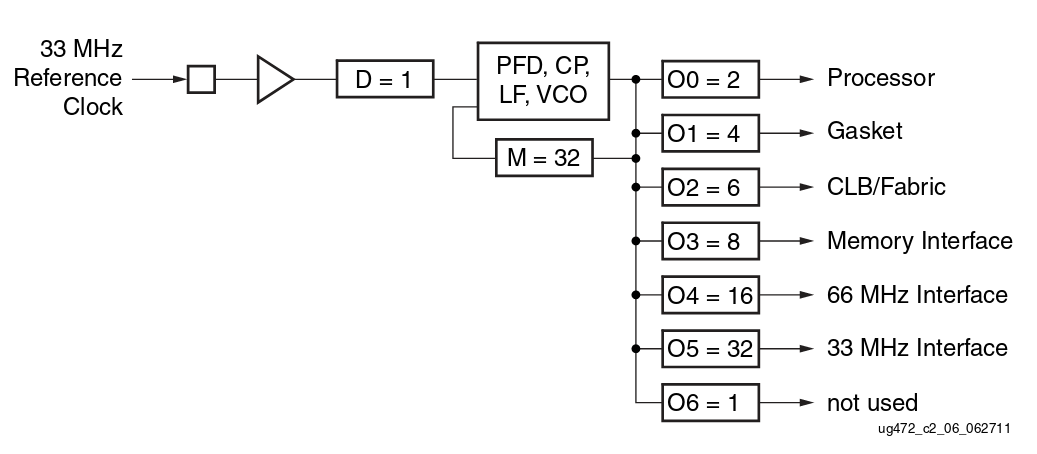
\includegraphics[scale=0.43]{mmcm_freq_synthesis.png}
  \captionof{figure}{ Использование MMCM в качестве генератора тактовых сигналов }
  \label{fig:functional:axi_clkgen:mmcm_freq_synthesis}
\end{center}

В качестве опорного тактового сигнала может выступать кварцевый генератор, или выходные
сигналы другого MMCM. Счётчик M (\en{Multiply}) задаёт коэффициент умножения опорной частоты.
Так же существует поддержка деления опорной частоты на дробный коэффициент. В режиме
деления частоты на дробное число конфигурирование скважности сигнала не поддерживается.

Если основной целью служит минимизация джиттера, то MMCM предоставляет самостоятельный
функциональный блок по фильтрации сигнала, который может применяться в любом месте
пайплайна генерации сигнала или при произвольной обработки. Для упрощения, можно считать, что
фильтр работает в качестве буффера, регенерирующего принимаемый сигнал с задаваемой частотой.

Блок  MMCM располагается как можно ближе к портам ввода-вывода, тем самым сокращая путь генерируемого тактового сигнала.
При этом MMCM может служить в качестве генератора произвольной частоты и для внутренней логики микросхемы.
Расположение MMCM в рамках микросхемы Artix-7 представлено на рисунке~\ref{fig:functional:axi_clkgen:mmcm_placement}

\begin{center}
  \centering
  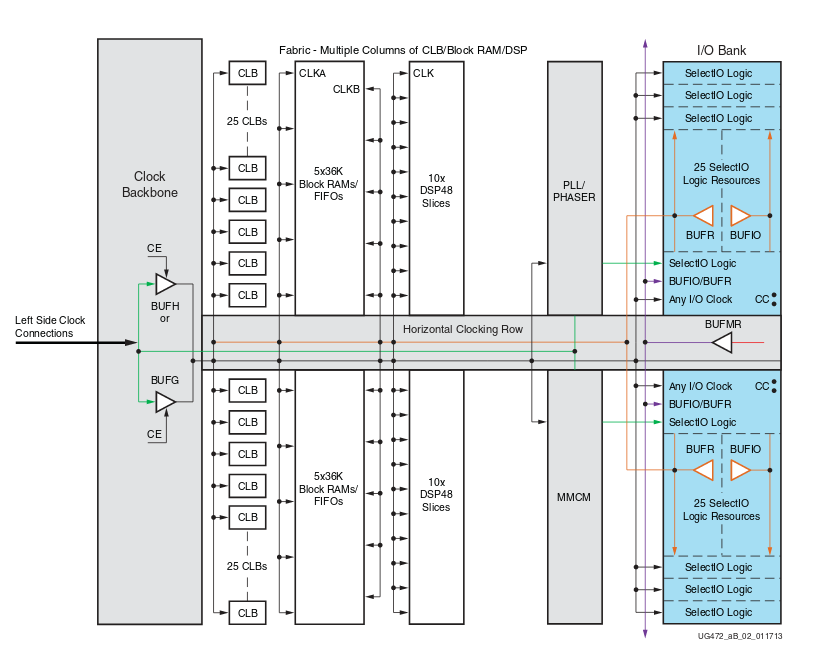
\includegraphics[scale=0.5]{mmcm_placement.png}
  \captionof{figure}{ Структурная схема MMCM }
  \label{fig:functional:axi_clkgen:mmcm_placement}
\end{center}

\subsection{AXI HDMI TX}
\label{sec:functional:axi_hdmi_tx}

Управление контроллером \en{HDMI} и передача данных на интерфейс может осуществлятся как напрямую,
так и при помощи специализированных IP-ядер от производителя контроллера. Ручной подход состоит из
проектирования блока на HDL языке по приёму видео в формате AXI4-Stream и его последующего отображения
на ножки контроллера HDMI. Часто производители контроллеров, интегрируемых на отладочные платы, предоставляют
доступ не только к документации и руководствам по эксплуатации их устройств, но и набором библиотек для
ускорения работы разработчика, путём переиспользования кода. В данном случае используется IP-ядро
от компании-производителя контроллера \en{AXI HDMI TX}.

Блок обладает следующим перечнем возможностей:
\begin{itemize}
  \item поддержка семейства протоколов AXI;
  \item поддержка разрешения видео вплоть до 1080p;
  \item передача видео по 36, 24 и 16-битным каналам;
  \item поддержка \en{emdedded sync};
  \item передача видео в цветовых пространствах YCbCR или RGB;
  \item клиппинг видеопотока.
\end{itemize}

AXI HDMI TX подготавливает передаваемый на порт видеопоток, после чего на основании
характеристик потока и начальной конфигуарции генерируются синхросигналы. Структурная схема
блока представлена на рисунке~\ref{fig:functional:axi_hdmi_tx:structure}

\begin{center}
  \centering
  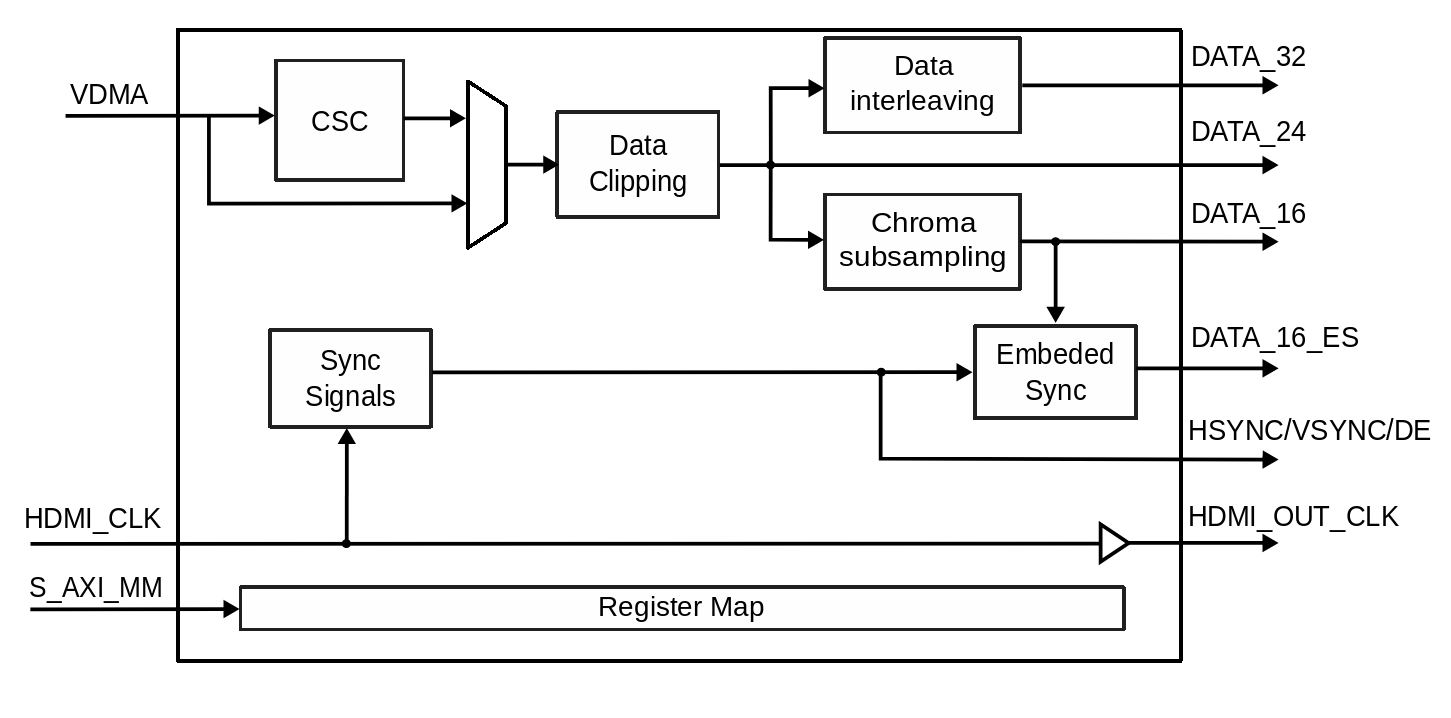
\includegraphics[scale=0.32]{axi_hdmi_tx.png}
  \captionof{figure}{ Структурная схема AXI HDMI TX }
  \label{fig:functional:axi_hdmi_tx:structure}
\end{center}

Конфигурируемые параметры блока:
\begin{itemize}
  \item ID --- должен быть уникален для каждого AXI HDMI TX в системе;
  \item DEVICE\_TYPE --- уникален для каждой отладочной платы и микросехмы;
  \item CR\_CB\_N --- используется в процессе цветовой субдискретизации, указывая
    какую цветовую компоненту в видеопотоке следует поместить между зелёными сэмплами;
  \item EMBEDDED\_SYNC --- активация режима \en{embedded sync};
  \item OUT\_CLOCK\_POLARITY --- выбор фронта тактового импульса.
\end{itemize}

Описание сигналов общего назначения блока приведено в таблице~\ref{table:functional:axi_hdmi_tx:common_signals}

\begin{table}[ht!]
  \caption{Описание сигналов общего назначения блока AXI HDMI TX}
  \label{table:functional:axi_hdmi_tx:common_signals}
  \begin{tabular}{| >{\centering}m{0.18\textwidth}
                  | >{\centering}m{0.17\textwidth}
                  | >{\centering\arraybackslash}m{0.57\textwidth}|}
   \hline
    Обозначение сигнала & Разрядность & Краткое описание \\
    \hline
    HCLK & 1 & Сигнал прорисовки пикселя, генерируется AXI CLKGEN \\
    \hline
    C & 1 & Сигнал тактирования HDMI контроллера \\
    \hline
    AXI4-Lite & --- & Сигналы шины AXI4-Lite, см. таблицу~\ref{table:functional:vmda_in:common_signals} \\
    \hline
  \end{tabular}
\end{table}

Так как блок поддерживает различные версии протокола HDMI с разной разрядностью
шины данных, то описание приведено исклюительно для используемой в данном проекте конфигурации.
Описание видеосигналов и сигналов контроллера HDMI приведено в таблице~\ref{table:functional:axi_hdmi_tx:signals}

\begin{table}[ht]
  \caption{Описание видеосигналов блока AXI HDMI TX}
  \label{table:functional:axi_hdmi_tx:signals}
  \begin{tabular}{| >{\centering}m{0.18\textwidth}
                  | >{\centering}m{0.17\textwidth}
                  | >{\centering\arraybackslash}m{0.57\textwidth}|}
   \hline
    Обозначение сигнала & Разрядность & Краткое описание \\
    \hline
    VDAT & 64 & Видеоданные \\
    \hline
    VALID & 1 & Валдиность принимаемых видеоданных \\
    \hline
    RDY & 1 & Сигнал разрешения приёма данных \\
    \hline
    FSRET & 1 & FSYNC \\
    \hline
    ARST & 1 & Сигнал сброса \\
    \hline
    VCLK & 1 & Тактирующий сигнал VDMA, позволяет развязать тактирующие цепи внутренней логики блока
               и передачи данных на контроллер \\
    \hline
    ACLK & 1 & Сигнал тактирования блока \\
    \hline
    D & 24 & Видеоданные, поступающие на HDMI контроллер после прохождения всех этапов обработки \\
    \hline
    HSYNC & 1 & Сигнал горизонтальной синхронизации \\
    \hline
    VSYNC & 1 & Сигнал вертикальной синхронизации \\
    \hline
    DE & 1 & Сигнал разрешения передачи данных \\
    \hline
    FSYNC & 1 & Самосинхронизация сигнала FSYNC, может использоваться для стабилизации
    частоты кадров\\
    \hline
  \end{tabular}
\end{table}


Так как протокол HDMI поддерживает передачу как видео, так и аудио, то для передачи
аудиосигнала необходимо использовать блок \en{AXI SPDIF TX}, позволяющий
передать на контроллер аудиосигнал, ввиду физической разделенности видео и аудиопотоков.

Источником видеопотока для блока служит \en{VDMA OUT}, передавая считанные из оперативной памяти
кадры на \en{AXI4-Stream} интерфейс. Синхронизация двух блоков осуществляется путём использования
общего тактового сигнала и сигналов кадровой синхронизации. В качестве тактового сигнала HDMI контроллера
выступает сигнал, генерируемый ядром AXI CLKGEN.

\subsection{AXI CAMERA I2C}
\label{sec:functional:axi_camera_i2c}

Основным источником и передатчиком данных в системе являются CMOS-камера и HDMI интерфейс.
Устройства являются внешними по отношению к микросхеме, поэтому для их управления необходимо использовать
какой-либо протокол связи. В основном производитель снабжает устройство достаточно простыми, с точки зрения
схемотехники, и популярными шинами: I2C, SPI, 1-Wire, CAN. Конфигурация и контроль состояния устройства не требует
большой пропускной способности шины, поэтому в этих целях используют последовательные шины.

Одним из самых популярных протоколов является I2C, ввиду его простоты, малого количества линий и большой
дальности передачи данных. Большинство производителей периферии оснащают её I2C контроллером, поэтому
для взаимодействия с ней в FPGA используется soft-контроллер, а не отдельный физический контроллер, распаянный
на плате.

Так как камера не входит в периферию платы, то она требует подключения через высокоскоростные разъёмы FMC.
Внутренняя разводка платы не предполагает изначального подключения каких-либо выводов микросхемы и периферии
платы к портам общего назначения, поэтому для управления камерой требуется развести цепи I2C к контактам контроллера I2C CMOS-камеры.

Использование распаянного на плате контроллера привело бы к необходимости физически соединить
контакты камеры на FMC разъёме и контакты контроллера. Однако soft-контроллер позволяет использовать
выводы микросхемы в качестве контактов, не требуя внесения изменений в отладочную плату.

Основные возможности блока I2C:
\begin{itemize}
  \item доступ к регистрам управления по шине AXI4-Lite;
  \item работа в master-slave режиме;
  \item поддержка режима multi master;
  \item программный выбор бита подтверждения;
  \item поддержка прерываний потери арбитража и определения адреса вызывающего устройства;
  \item генерация START и STOP сигналов;
  \item генерация сигнала START с повторением;
  \item генерация и обнаружение бита подтверждения;
  \item автоматическое определение занятости шины;
  \item поддержка режимов \en{Fast-Mode Plus, Fast Mode} и \en{Standard Mode};
  \item 7-битная или 10-битная адресация;
  \item FIFO для приёма и передачи;
  \item динамическая генерация START и STOP сигналов;
\end{itemize}

Данное ядро не предоставляет явных связей с шиной I2C, поэтому подключение к шине организоывается
самостоятельно. Необходимо присутствие двунаправленных буферов ввода-вывода в контроллере шины,
управляющий линиями SDA и SCL с открытым коллектором. В различных случаях может потребоваться
установка подтягивающих резисторов, для поддержания стабильного высокого уровня при отключении
драйвера шины. Значения сопротивлений подбираются согласно технической документации к подключаемому
устройству, в данном случае это спецификация CMOS-камеры. Если таковая отсутствует, то расчёт
производится согласно стандарту протокола I2C.

Структурная схема блока представлена на рисунке~\ref{fig:functional:axi_camera_i2c:structure}

\begin{center}
  \centering
  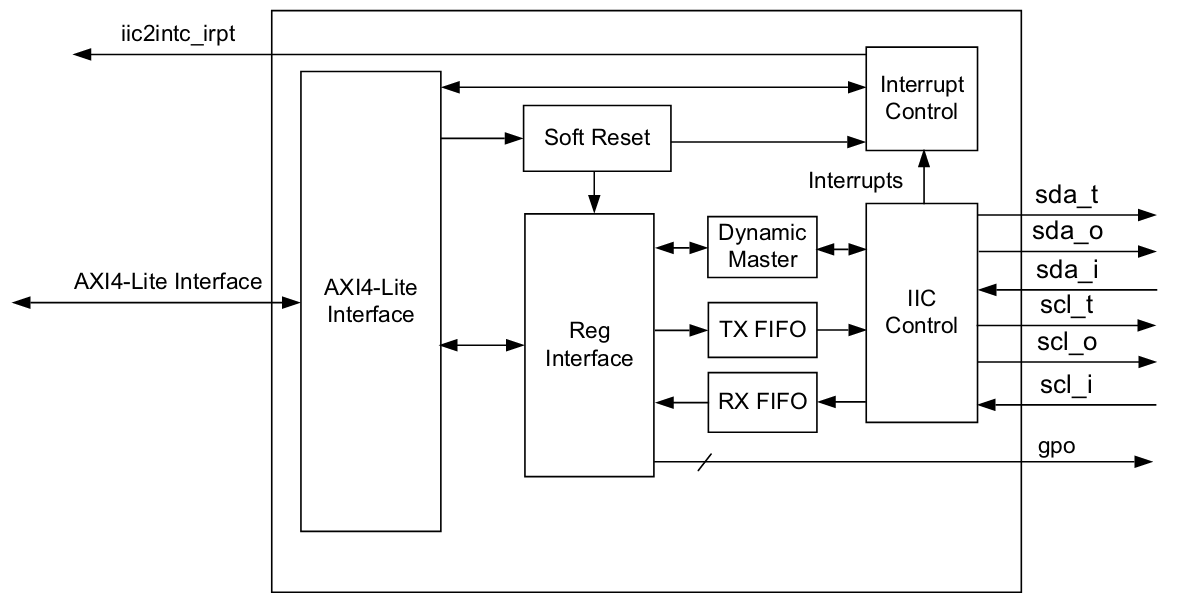
\includegraphics[scale=0.38]{i2c.png}
  \captionof{figure}{ Структурная схема AXI CAMERA I2C }
  \label{fig:functional:axi_camera_i2c:structure}
\end{center}

Блок разбит на несколько модулей:
\begin{itemize}
  \item AXI4-Lite Interface --- реализует одноимённый протокол, оперирует в режиме slave, используется
    для доступа к внутренним регистрам блока;
  \item Interrupt Control --- отслеживает статус прерываний блока и генерирует хост-прерывания;
  \item Registers Interface --- содержит управляющие регистры и регистры статуса. Имеет доступ к
    \en{TX FIFO} и \en{RX FIFO}. Доступ к регистрам осуществляется через AXI4-Lite интерфейс;
  \item TX, RX FIFO --- буферизация передаваемых или принимаемых данных;
  \item Dynamic Master --- динамически контролирует режим работы блока, начинает работу при записи
    старт и стоп битов в буфер передатчика;
  \item Soft Reset --- позволяет программно сбросить состояние блока;
  \item IIC Control --- конечный управляющий автомат шины I2C, связан с модулем \en{Dynamic Master} для
    переключения состояния блока в \en{master} или \en{slave};
  \item \en{Dynamic I2C Controller Logic} --- HAL, можнт работать в режиме мастера с 7-битной адресацией.
\end{itemize}

При наличии нескольких master устройств на одной шине блок оперирует в режиме \en{Multi-Master}.
Блок участвует в процессе арбитража только в том случае, когда шина свободна. Ядро
выставляет последовательность START, после чего другие master устройства на шине
присоединяются к арбитражу. Ядро корректно отрабатывает передачу шины
устройству с меньшим адресом на шине. Если шина не свободна, что определяется
по низкому уровню линии SDA и высокому SCL, то блок ждёт следующей возможности
захватить шину.

При работе шины в режиме \en{Fast Mode}, согласно спецификации I2C, требуется применять
фильтр низких частот для подавления высокочастотных всплесков на линии SCL. Фильтр
может настраиваться на импульсы от 0 до 50 наносекунд, задавая ширину полосы
в количестве тактовых импульсов. Некоторые устройства могут не требовать применния фильторв,
другие же применения максимально узкой полосы даже при работе в самом низкочастотном режиме.
При необходимости подавлять всплески длиной более 50 нс. требуется дополнительное согласование
со спецификацией.

Описание сигналов блока приведено в таблице~\ref{table:functional:axi_camera_i2c:signals}

\begin{table}[ht!]
  \caption{Описание сигналов блока AXI CAMERA I2C}
  \label{table:functional:axi_camera_i2c:signals}
  \begin{tabular}{| >{\centering}m{0.18\textwidth}
                  | >{\centering}m{0.17\textwidth}
                  | >{\centering\arraybackslash}m{0.57\textwidth}|}
   \hline
    Обозначение сигнала & Разрядность & Краткое описание \\
    \hline
    AXI4-Lite & --- & Сигналы шины AXI4-Lite \\
    \hline
    SDAI & 1 & Последовательный приём данных из буфера с тремя состояниями \\
    \hline
    SDAO & 1 & Последовательная передача в буфер с тремя состояниями \\
    \hline
    SDAT & 1 & Разрешение на передачу данных в буфер с тремя состояниями \\
    \hline
    SCLI & 1 & Приём тактового сигнала из буфера с тремя состояниями \\
    \hline
    SCLO & 1 & Передача тактового сигнала в буфер с тремя состояниями \\
    \hline
    SCLT & 1 & Разрешение на передачу тактового сигнала в буфер с тремя состояниями \\
    \hline
  \end{tabular}
\end{table}

Блок AXI CAMERA I2C подключается по шине AXI4-Lite к микропроцессору, который
проводит инициализацию блока и с его помощью управляет контроллером камеры.
Линии шины I2C подключены к контроллеру I2C модуля CMOS-камеры. При помощи блока
конфигурируется камера, после чего активируется передача кадров в систему.

\subsection{AXI HDMI I2C}
\label{sec:functional:axi_hdmi_i2c}

Описание данного блока схоже с \en{AXI HDMI I2C}, за исключением того, что
блок позволяет микропроцессору настраивать HDMI контроллер и отслеживать его состояние
в процессе передачи, тем самым позволяя сменять режимы работы во время работы устройства,
не перезагружая всю систему в целом.

\subsection{AXI UART-Lite }
\label{sec:functional:axi_uart_lite}

В процессе разработки неоднократно возникает необходимость получения отладочной
информации и ведения логов. Так как использование отладчика решает только половину
проблемы, то для полноценной отладки можно использовать контроллер UART. Протокол
UART является достаточно популярным решением для отладки аппаратных платформ и устройств,
поэтому на них часто устанавливается не только контроллер, но и преобразователи
интерфейсов. На используемой в проекте плате установлен UART контроллер с преобразователем
в USB, позволяя достаточно тривиально подключаться к плате.

Схожий с I2C подход, позволяет не только обращаться к контроллеру по заранее подготовленным связям, но и
подключить любое UART-совместимое устройство к произвольным выводам, к которым микросхема может обращаться
при помощи IP-ядра.

Ядро AXI UART-Lite является soft-контроллером для связи по протоколу UART, связь с которым осуществляется
по \en{AXI4-Lite}. Блок поддерживает:
\begin{itemize}
  \item AXI4-Lite интерфейс для доступа к регистрам и передачи данных;
  \item полнодуплексный режим работы;
  \item 16-символьная очередь на приём и передачу;
  \item конфигурируемое число бит в символе (от 5 до 8);
  \item бит чётности (чётный, нечётный или выключен);
  \item задаваемый бодрейт.
\end{itemize}

Так как UART представляет собой последовательный интерфейс, а AXI4-Lite --- параллельный,
то при передаче символов осщуествляется конверсия из параллельного представления в
последовательное, и наборот при приёме.

Структурная схема блока приведена на рисунке~\ref{fig:functional:axi_uart_lite:structure}

\begin{center}
  \centering
  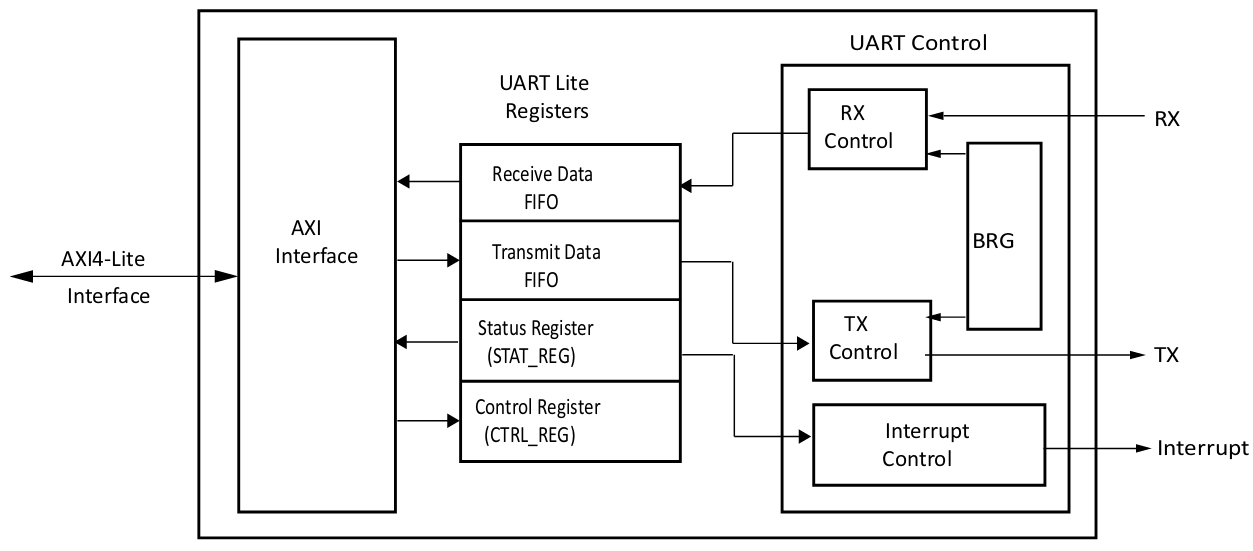
\includegraphics[scale=0.36]{uart_lite.png}
  \captionof{figure}{ Структурная схема AXI UART-Lite }
  \label{fig:functional:axi_uart_lite:structure}
\end{center}

При появлении элементов в очередях приёма или передачи генерируется прерывания,
которое может быть маскировано. Для установки бодрейта используется встроенный генератор,
который в качестве источника опорной частоты использует тактовый сигнал AXI4-Lite.

Блок регистров состоит из:
\begin{itemize}
  \item очереди приёмника;
  \item очереди передатчика;
  \item регистров состояния;
  \item управляющих регистров;
\end{itemize}

Регистры отображаются в память, обе очереди длиной в 16 символов.

Блок управления состоит из контроллера приёмника, контроллера передатчика,
генератора бодрейта и контроллер прерываний. Контроллер приёмника разбивает
принятные данные в виде последовательности бит на группы символов определенной
длины, в соответствии с бодрейтом, после чего сохраняет группу символов в
очереди приёмника. Блок управления передатчиком собирает данные из его очереди,
после чего посылает их на интерфейс TX. Контроллер бодрейта генерирует
бодрейт с заданным значением. Контроллер прерываний генерирует прерывания при
появлении данных в очереди, либо при её опустошении.

Описание сигналов блока приведено в таблице~\ref{table:functional:axi_uart_lite:signals}

\begin{table}[ht!]
  \caption{Описание сигналов блока AXI UART-Lite}
  \label{table:functional:axi_uart_lite:signals}
  \begin{tabular}{| >{\centering}m{0.18\textwidth}
                  | >{\centering}m{0.17\textwidth}
                  | >{\centering\arraybackslash}m{0.57\textwidth}|}
   \hline
    Обозначение сигнала & Разрядность & Краткое описание \\
    \hline
    AXI4-Lite & --- & Сигналы шины AXI4-Lite \\
    \hline
    TX & 1 & Порт передачи данных \\
    \hline
    RX & 1 & Порт приёма данных \\
    \hline
  \end{tabular}
\end{table}

Блок подключается к микропроцессору по шине AXI4-Lite для обмена отладочными данными
между компьютером и микропроцессором.

\subsection{MicroBlaze}
\label{sec:functional:microblaze}

В качестве микропроцессора, необходимого любому современному устройству, выбран процессор MicroBlaze.
MicroBlaze это soft-core микропроцессор, полностью реализуемый на базе логических элементов FPGA.
На данный момент это единственный поддерживаемый компанией Xilinx микропроцессор.

MicroBlaze представляет собой 32-битный RISC (\en{Reduced Instruction Set Computer}) процессор,
специально оптимизированный для реализации на базе логических блоков FPGA. Большая
часть внутренней структуры процессора может как включаться, отключаться, так и урезаться
по функциональности, если к системе существуют требования по быстродействию и энергопотреблению.

Схема процессора приведена на рисунке~\ref{fig:functional:microblaze:structure}

\begin{center}
  \centering
  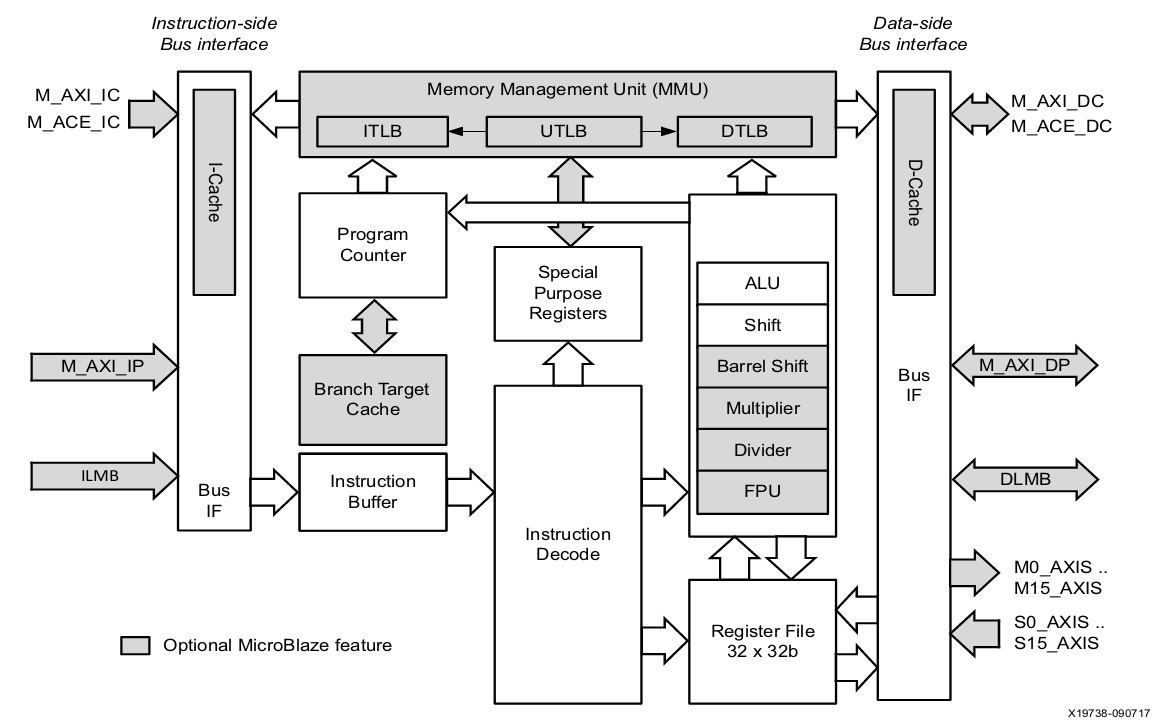
\includegraphics[scale=0.38]{microblaze.png}
  \captionof{figure}{ Структурная схема процессора MicroBlaze }
  \label{fig:functional:microblaze:structure}
\end{center}

Практически все блоки микропроцессора могут конфигурироваться, однако есть набор фиксированных
параметров:
\begin{itemize}
  \item длина регистров общего назначения в 32 бита;
  \item разрядность регистра инструкций составляет 32 бита;
  \item все инструкции трёхоперандные с двумя режимами адресации;
  \item шина адреса по-умолчанию составляет 32 бита, расширяема до 64;
  \item одно устройство выполнения в конвейере.
\end{itemize}

Микропроцессор может использовать \en{Big-Endian} или \en{Little-Endian} порядок байт,
аппаратно поддерживаемыми типами являются слово, полуслово и один байт

% 11 страница reference guide